\documentclass[12pt,onecolumn]{article}
\usepackage[utf8]{inputenc} % UTF8 input encoding
\usepackage[T2A]{fontenc}   % T2A font encoding for Cyrillic script
\usepackage[russian]{babel} % Russian language support
\usepackage{listings}
\usepackage{tikz}
\usepackage{aeguill}
\usepackage{float}
\usepackage{mathtools}
\everymath{\displaystyle}
\usepackage{listings} 
\usepackage{hyperref}
\usepackage{geometry}
\usepackage{verbatim}
\usepackage{amsmath}
\usepackage{multirow}
\usepackage{graphicx}
\newcommand{\nparagraph}[1]{\paragraph{#1}\mbox{}\\}
\geometry{
  a4paper,
  top=20mm, 
  right=20mm, 
  bottom=20mm, 
  left=25mm
}
\lstdefinestyle{verilog}{ 
  basicstyle=\small\ttfamily,
  commentstyle=\color{cyan},
  stringstyle=\color{magenta}\ttfamily,
  keywordstyle=\color{blue},
  numbers=left,
  numberstyle=\scriptsize,
  numbersep=5pt,
  frame=single,
  breaklines=true,
  breakatwhitespace=true,
  showstringspaces=false,
  tabsize=4,
  inputencoding=utf8,
  extendedchars=true
}

\begin{document}
\setcounter{tocdepth}{4}
\begin{center}
    Федеральное государственное автономное образовательное учреждение высшего образования "Национальный Исследовательский Университет ИТМО"\\ 
    Мегафакультет Компьютерных Технологий и Управления\\
    Факультет Программной Инженерии и Компьютерной Техники \\
    
\includegraphics[scale=0.3]{image/itmo.jpg} % нужно закинуть картинку логтипа в папку с отчетом
\end{center}
\vspace{1cm}


\begin{center}
    \large \textbf{Вариант №133211}\\
    \textbf{Лабораторная работа 2}\\
    по дисциплине\\
    \textbf{Тестирование программного обеспечения}
\end{center}

\vspace{2cm}

\begin{flushright}
  Выполнил Студент  группы P33102\\
  \textbf{Лапин Алексей Александрович}\\
  Преподаватель: \\
  \textbf{Харитонова Анастасия Евгеньевна}\\
\end{flushright}

\vspace{9cm}
\begin{center}
    г. Санкт-Петербург\\
    2024г.
\end{center}
\pagestyle{empty}

\pagestyle{plain}
\section*{Задание:}
\begin{figure}[H]
    \centering
    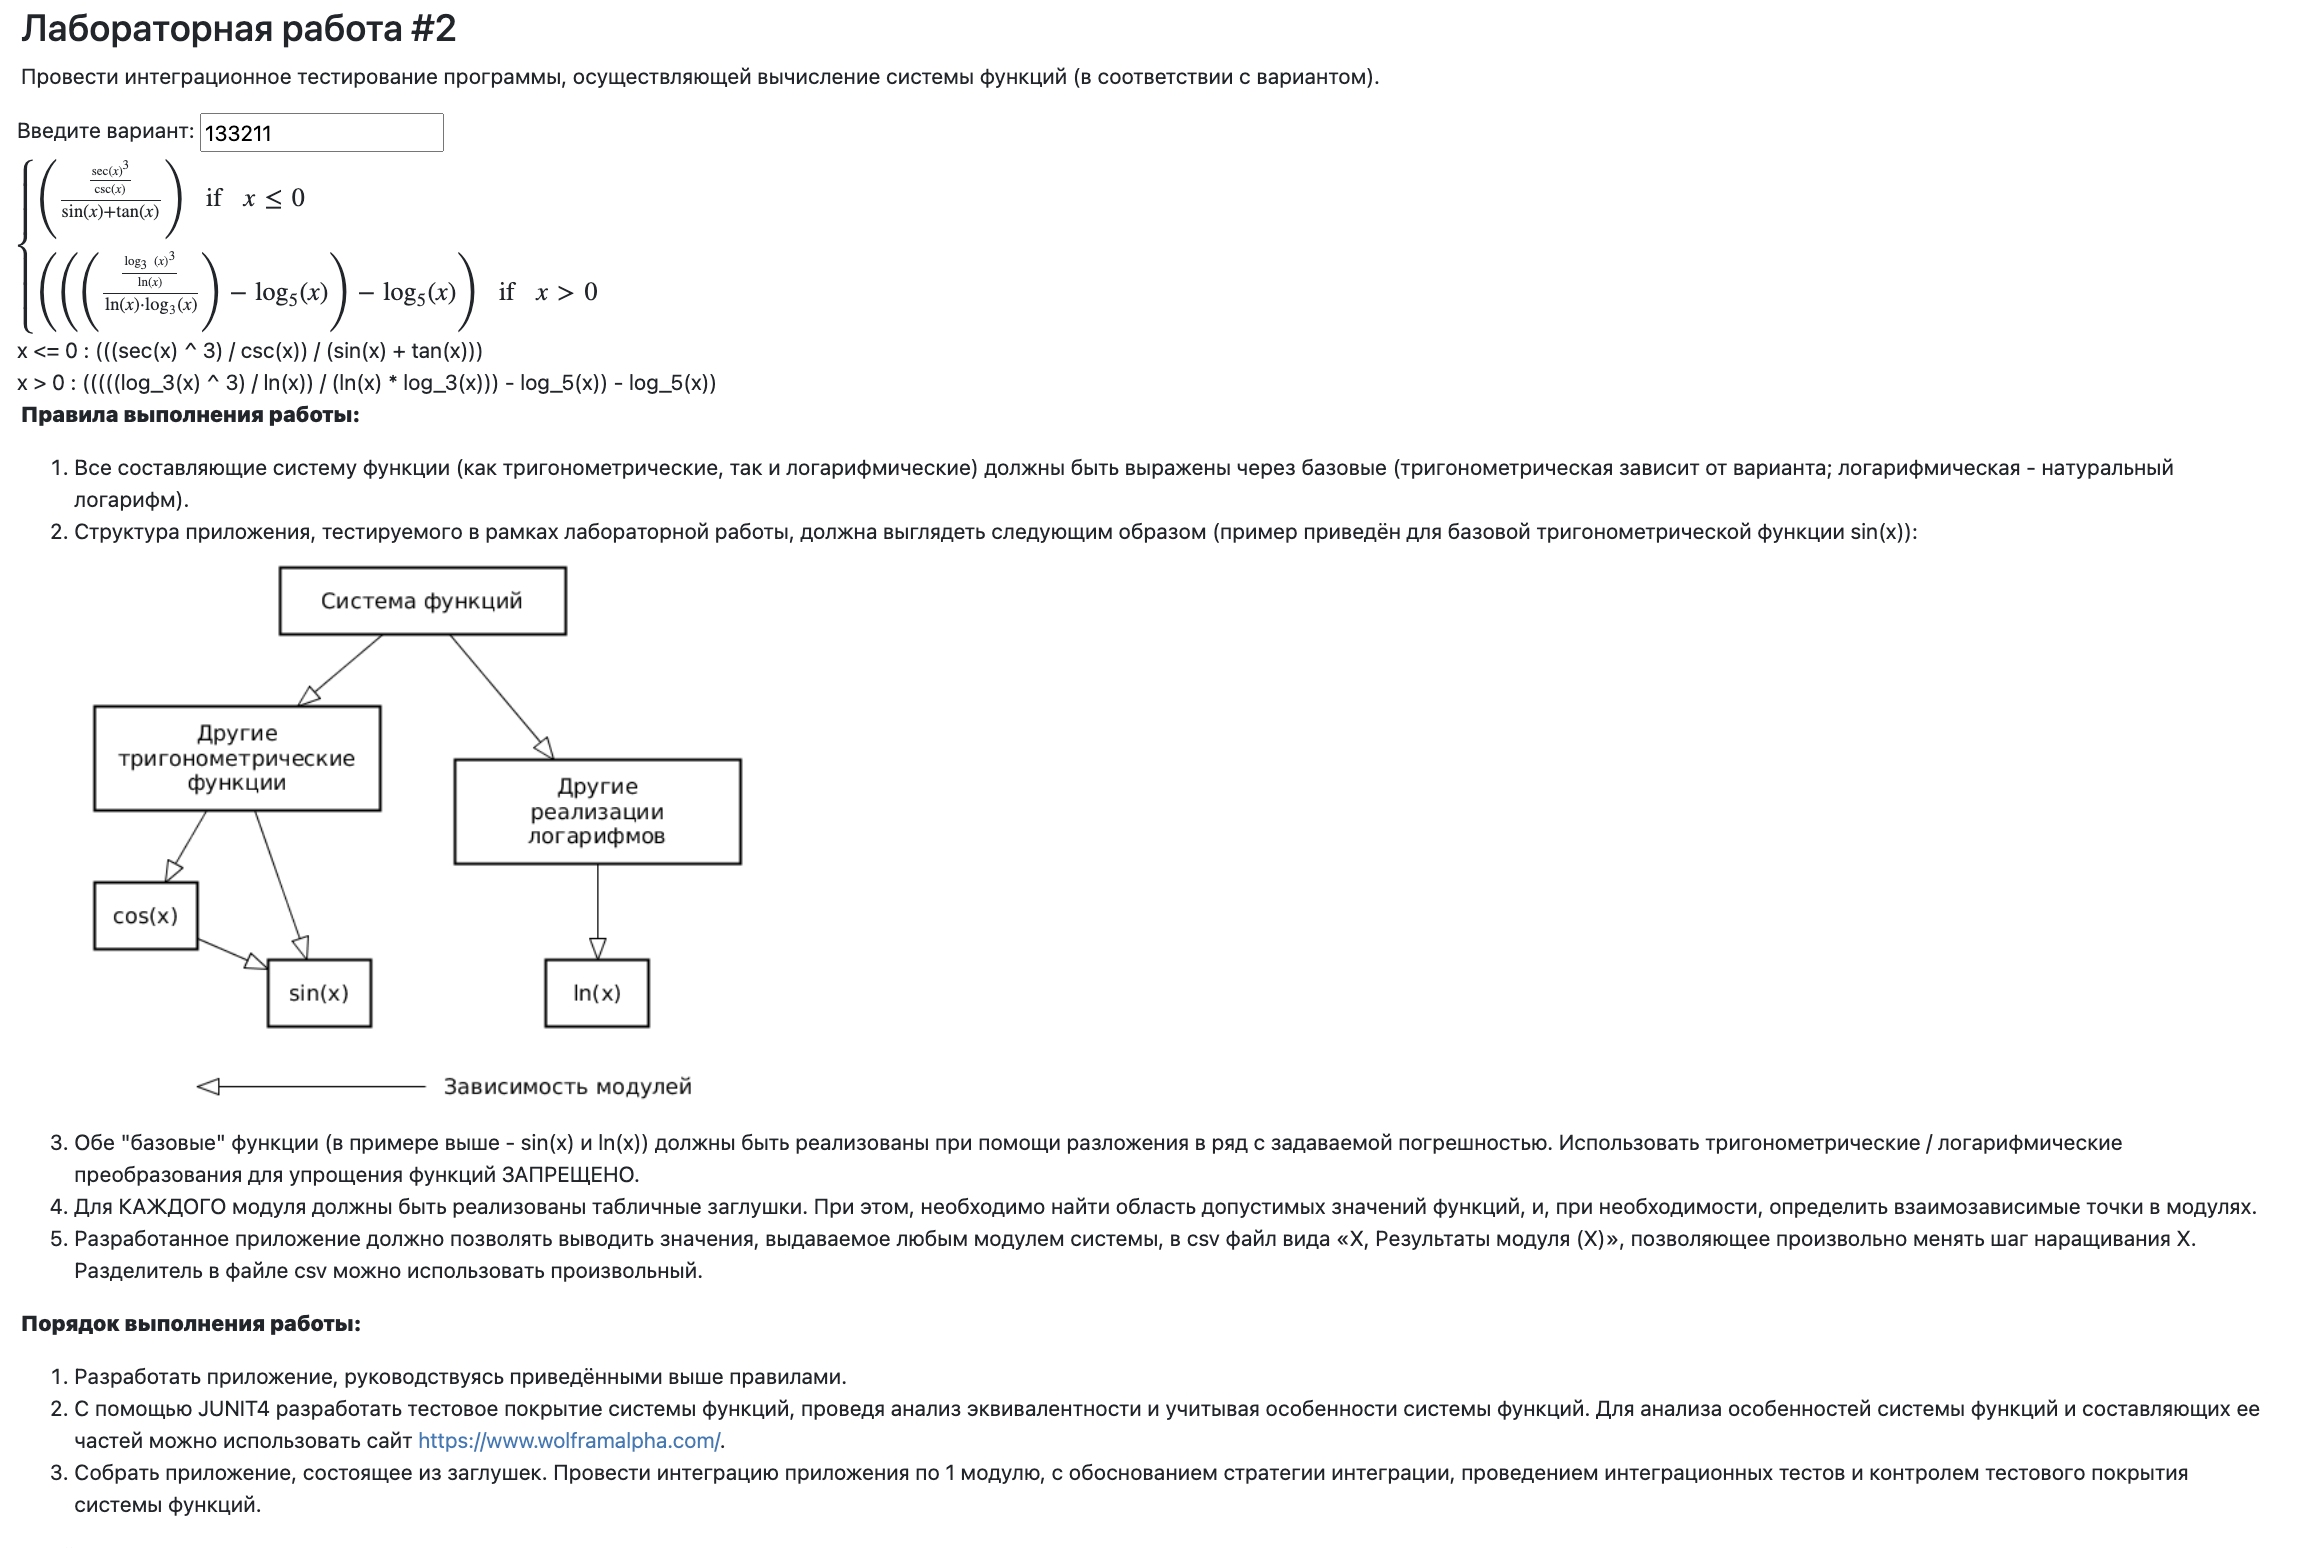
\includegraphics[width=\textwidth]{image/task.png}
\end{figure}
\section*{UML-диаграмма классов разработанного приложения.}
\begin{figure}[H]
    \centering
    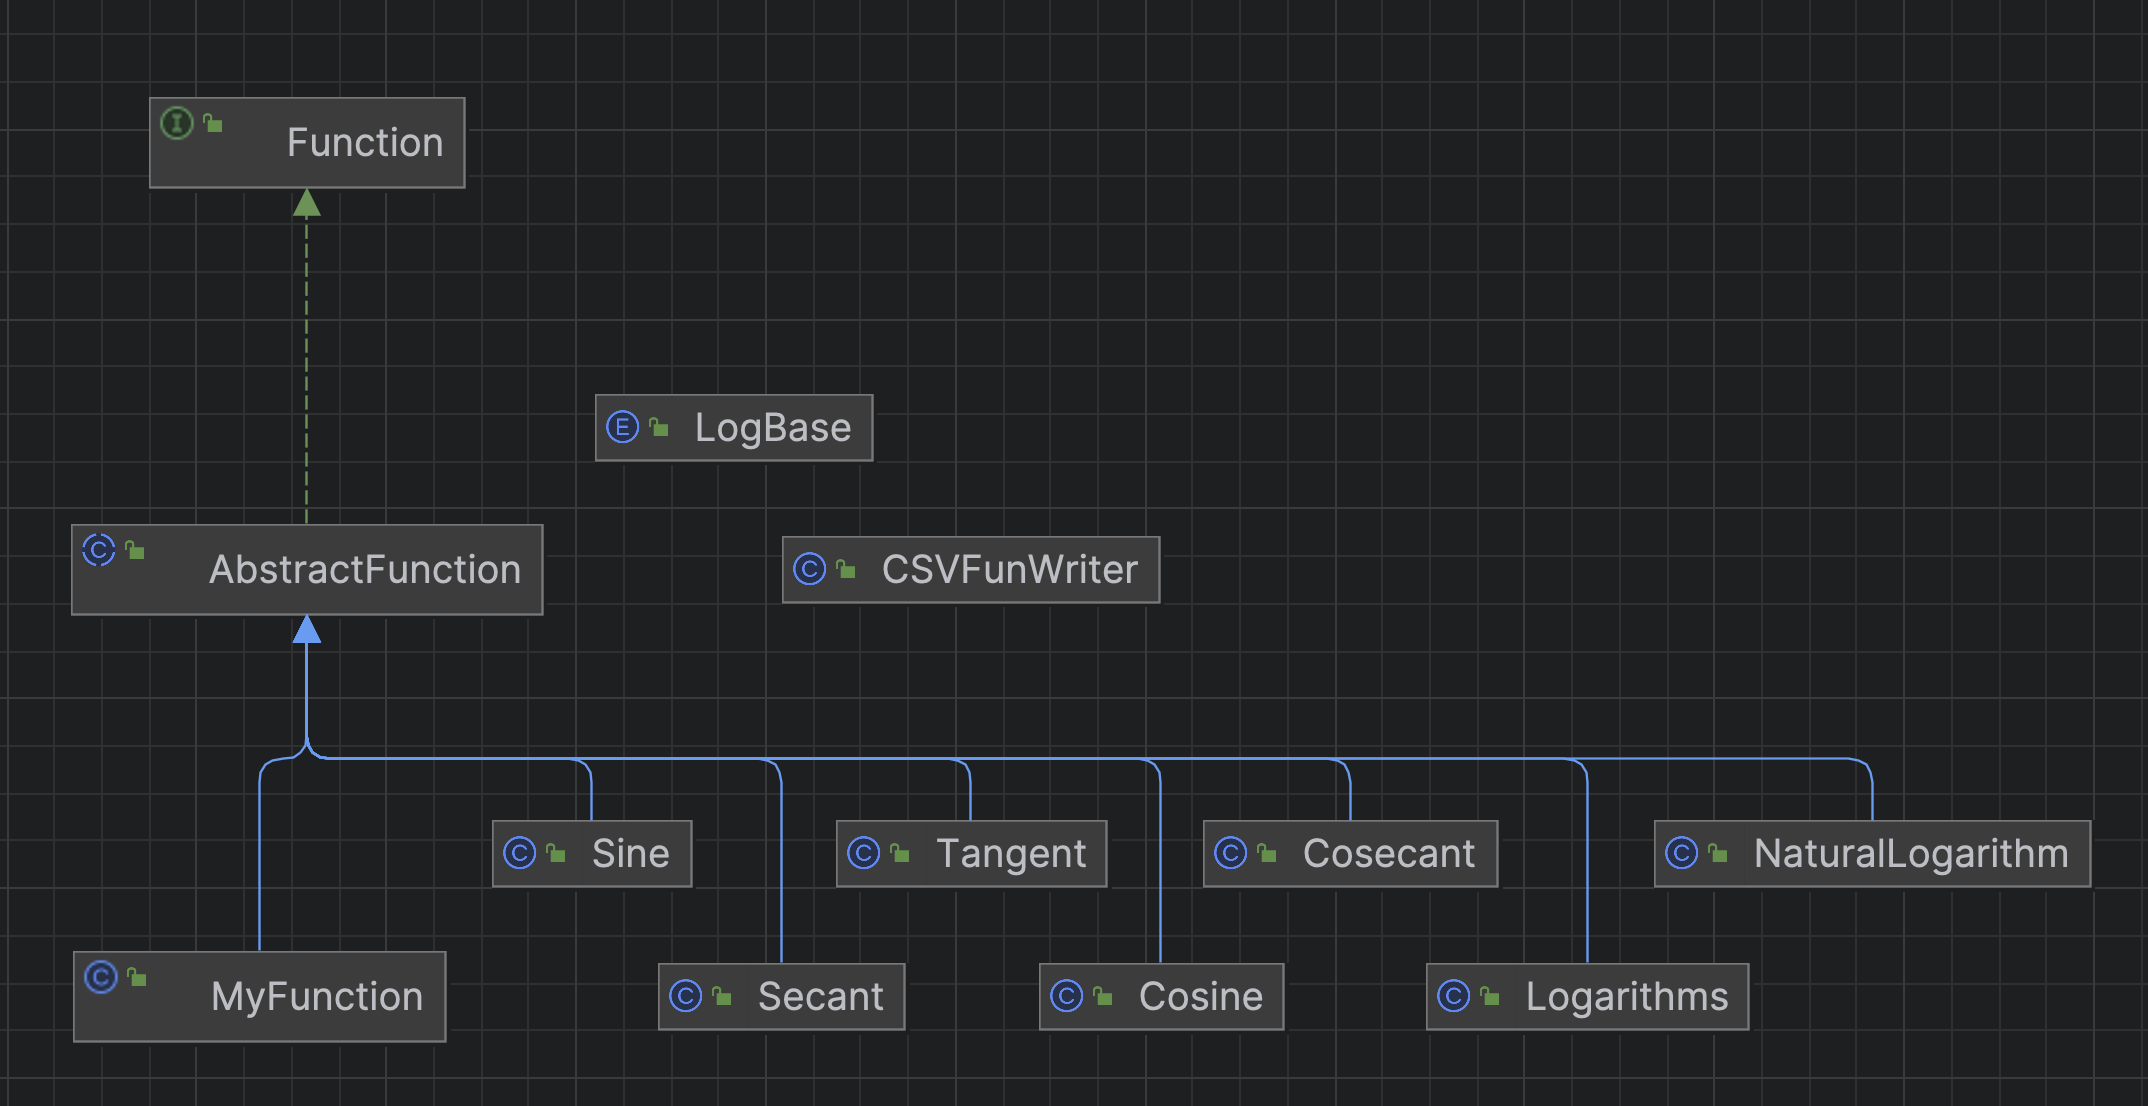
\includegraphics[width=\textwidth]{image/UML1.png}
\end{figure}
\begin{figure}[H]
    \centering
    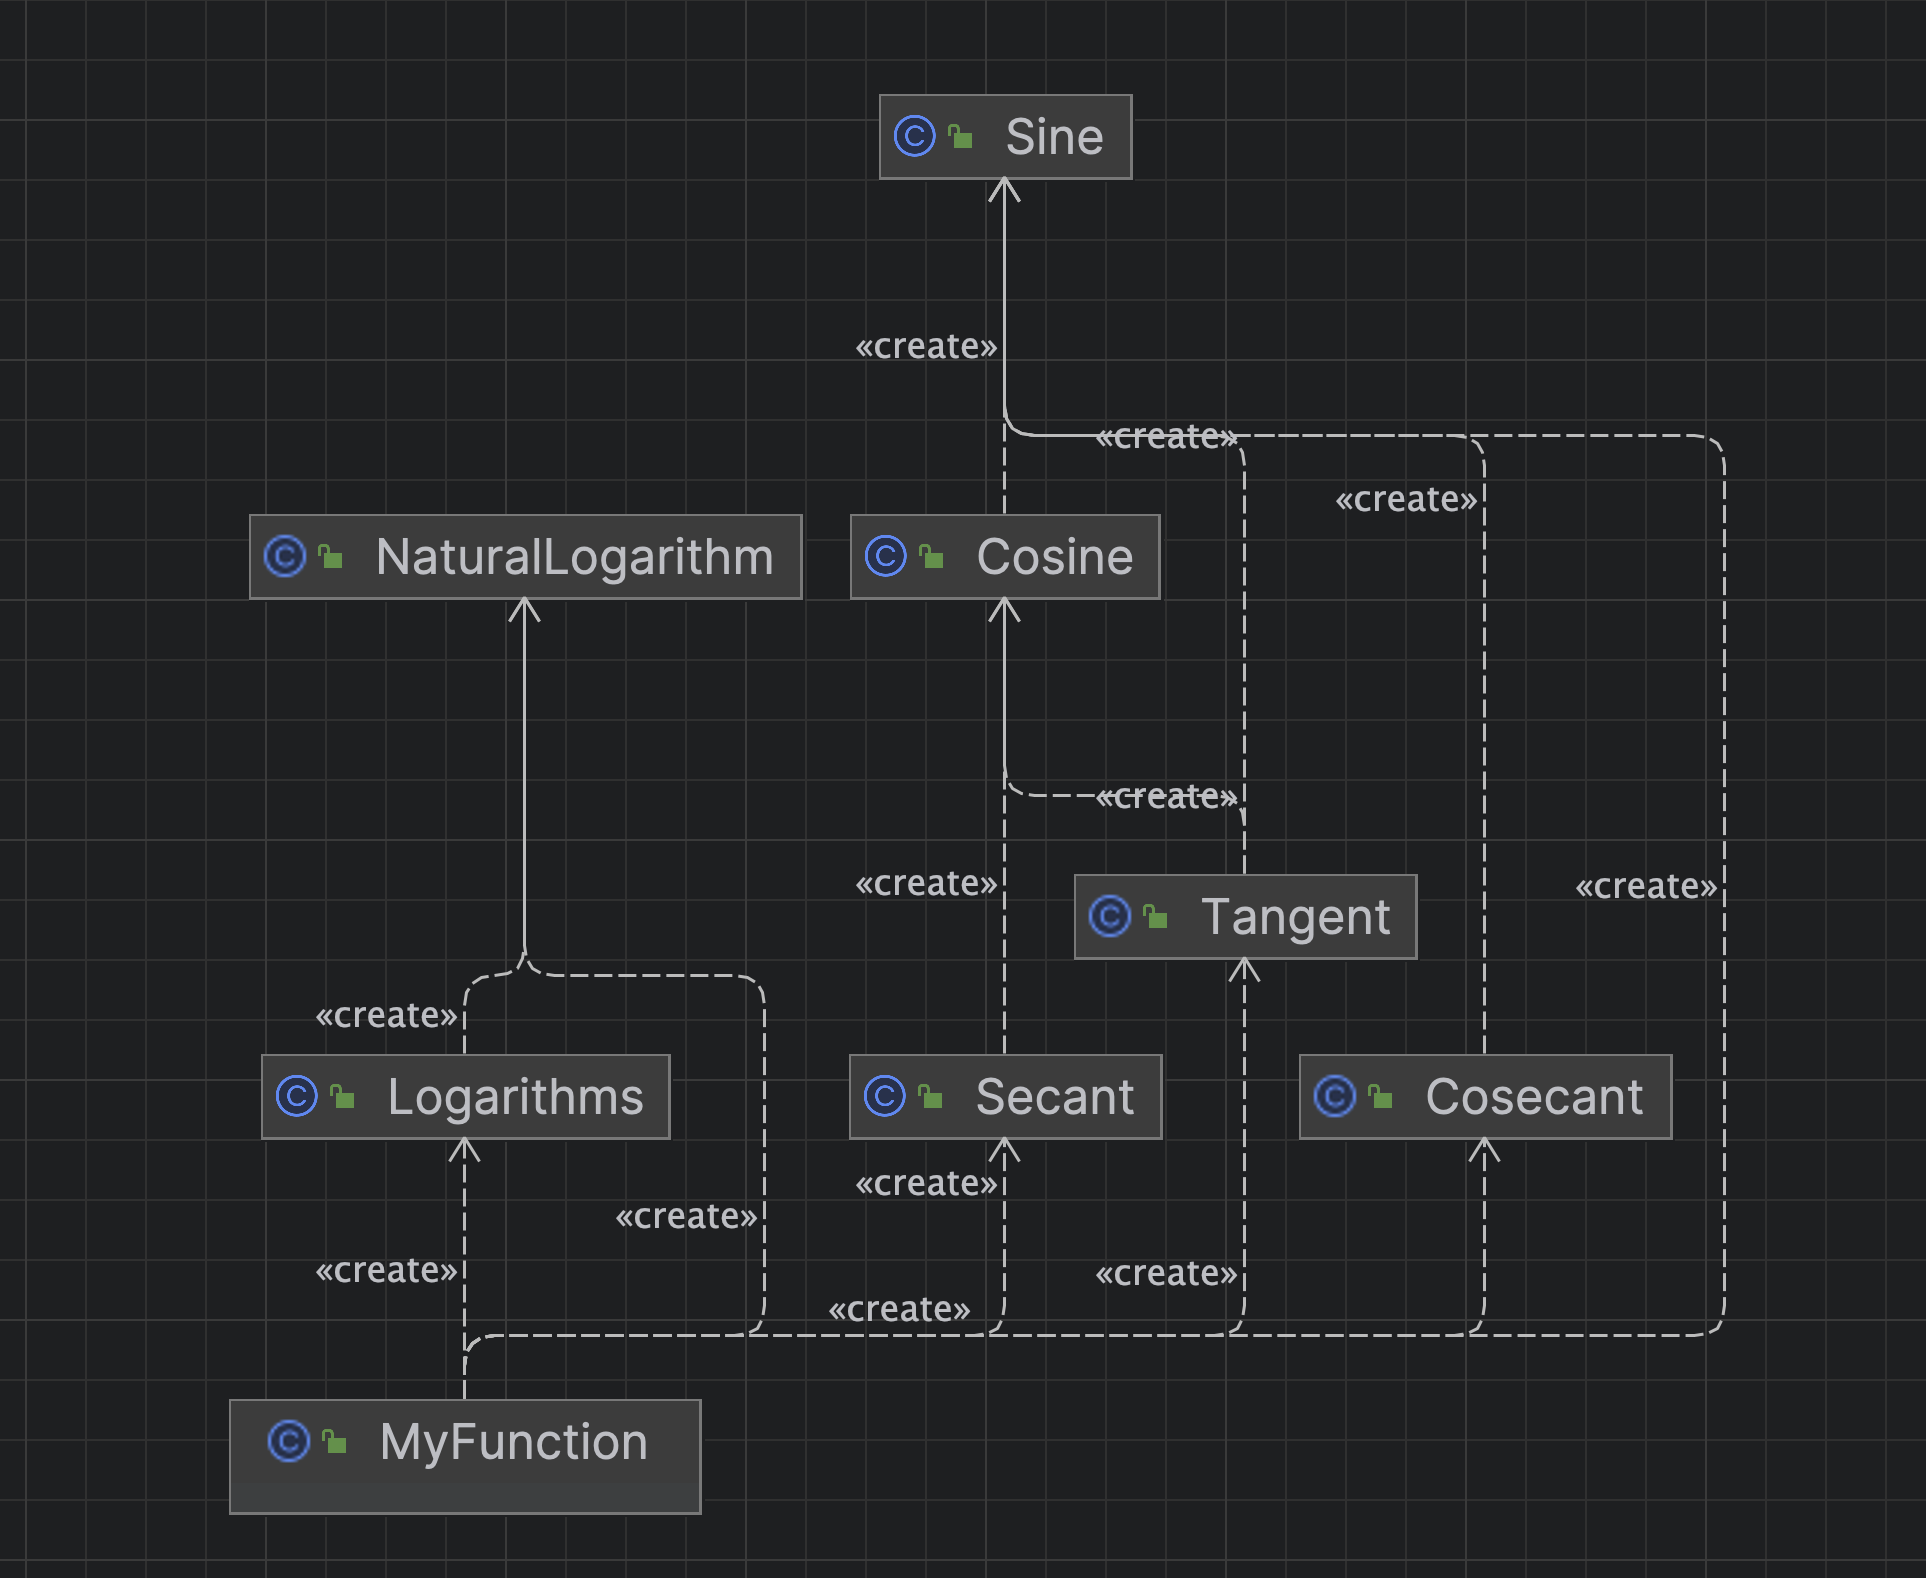
\includegraphics[width=\textwidth]{image/UML2.png}
\end{figure}
\section*{Описание тестового покрытия с обоснованием его выбора.}
\input{image/coverage.latex}

Интеграция приложения проводилась сверху вниз, так как этот метод позволяет использовать заглушки, которые гораздо проще реализовать и в целом данный вид интеграции более прост в реализации.
Тестовое покрытие состоит из 2 частей:
\begin{enumerate}
    \item Модульные тесты для каждого класса.
    \item Интеграционные тесты для проверки взаимодействия классов в MyFunction.
\end{enumerate}
\begin{figure}[H]
    \centering
    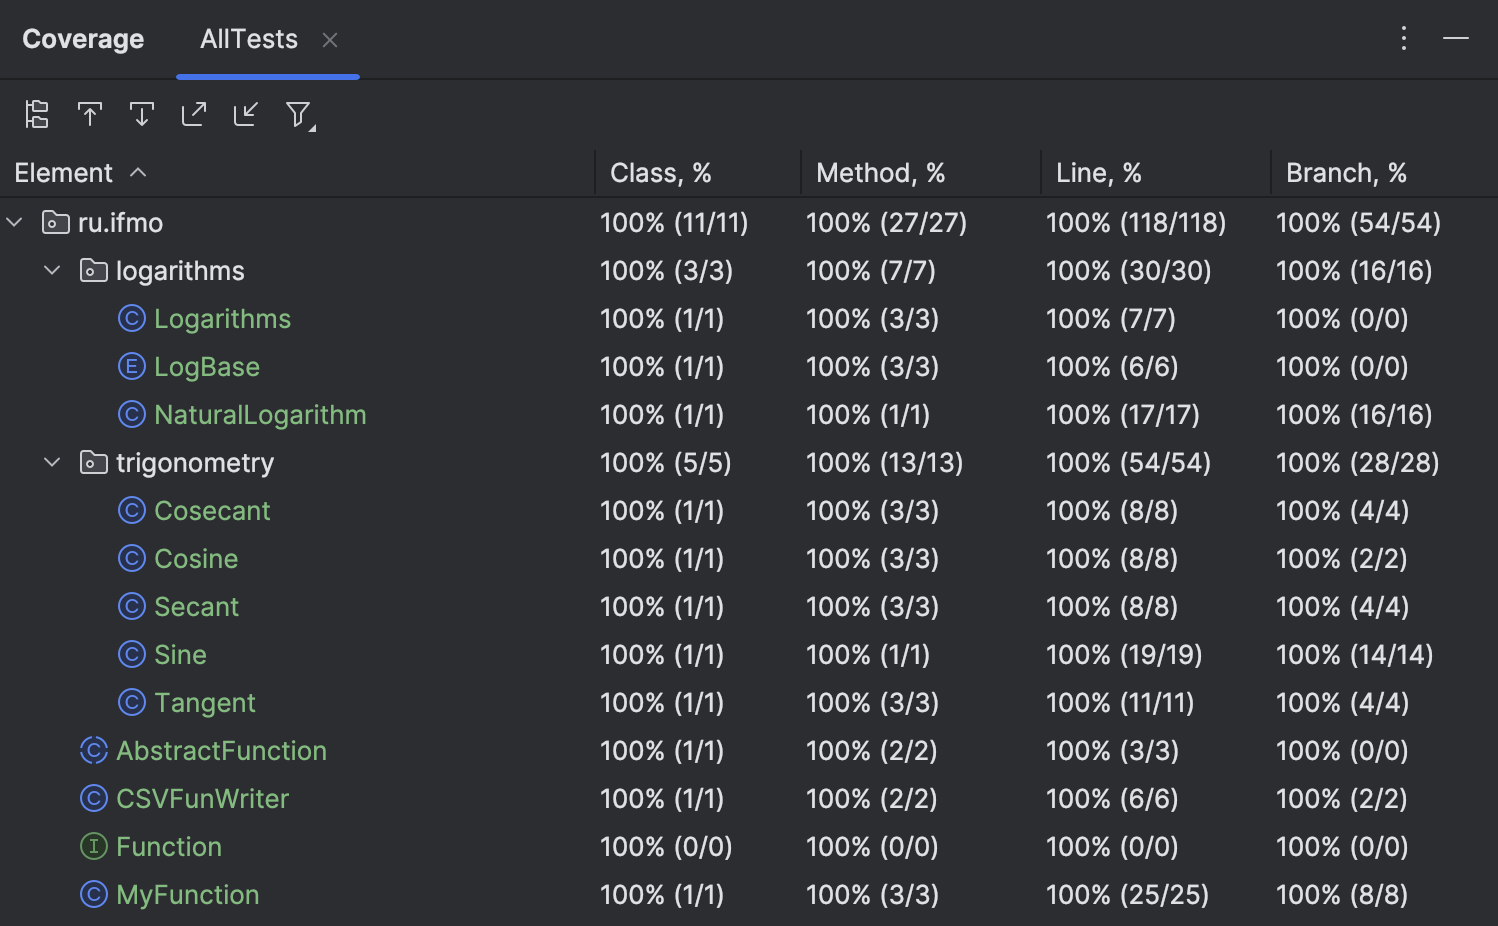
\includegraphics[width=\textwidth]{image/coverage.png}
\end{figure}
\section*{Графики, построенные csv-выгрузкам, полученным в процессе интеграции приложения.}
\begin{figure}[H]
    \centering
    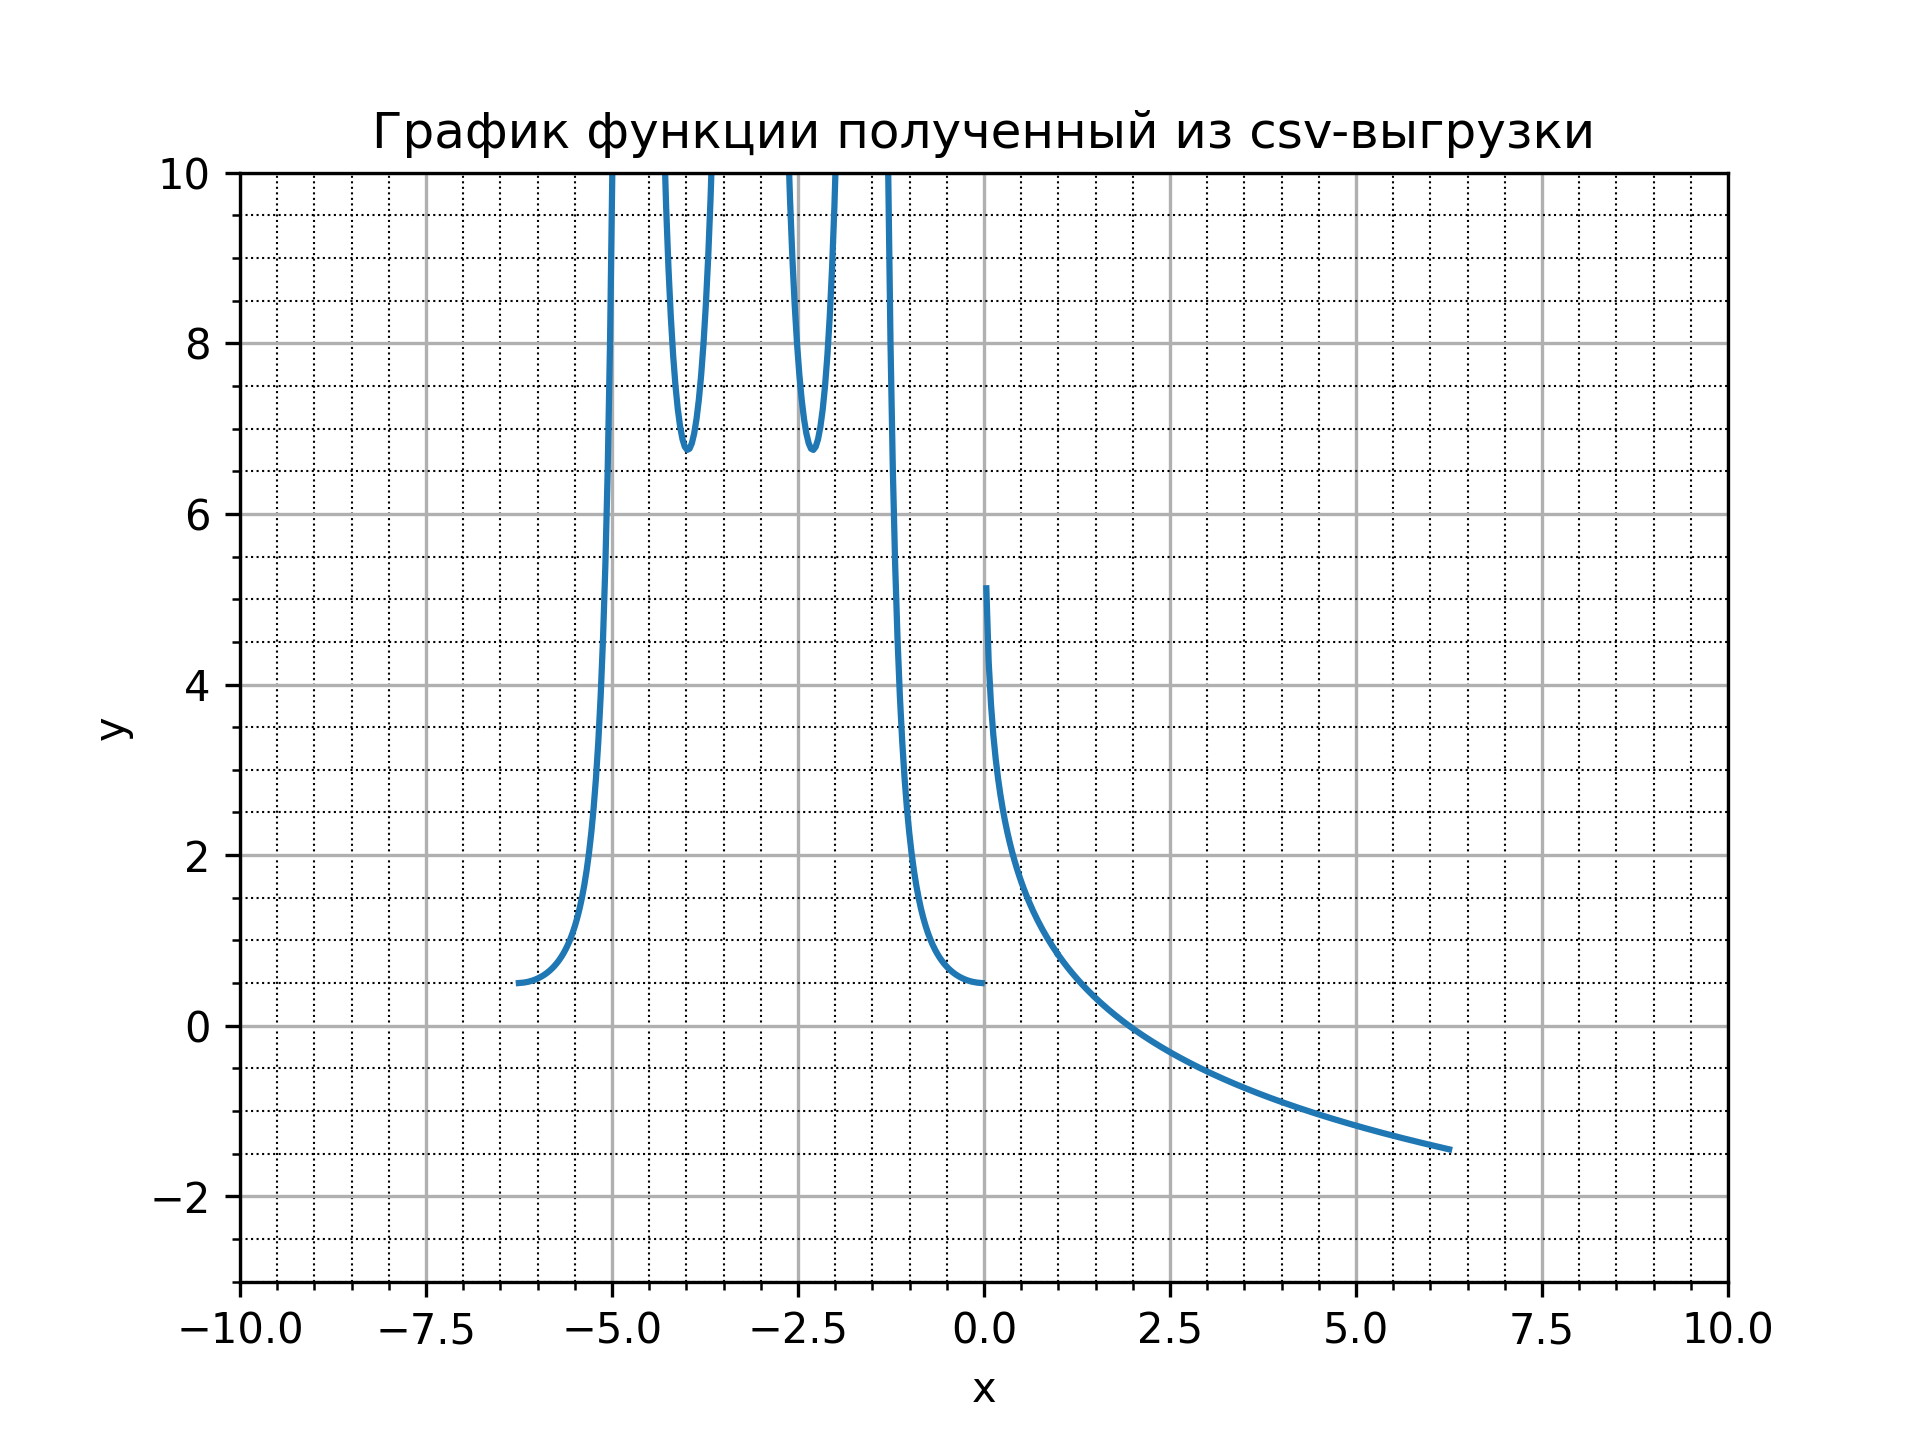
\includegraphics[width=\textwidth]{image/myFunc.png}
\end{figure}
\begin{figure}[H]
    \centering
    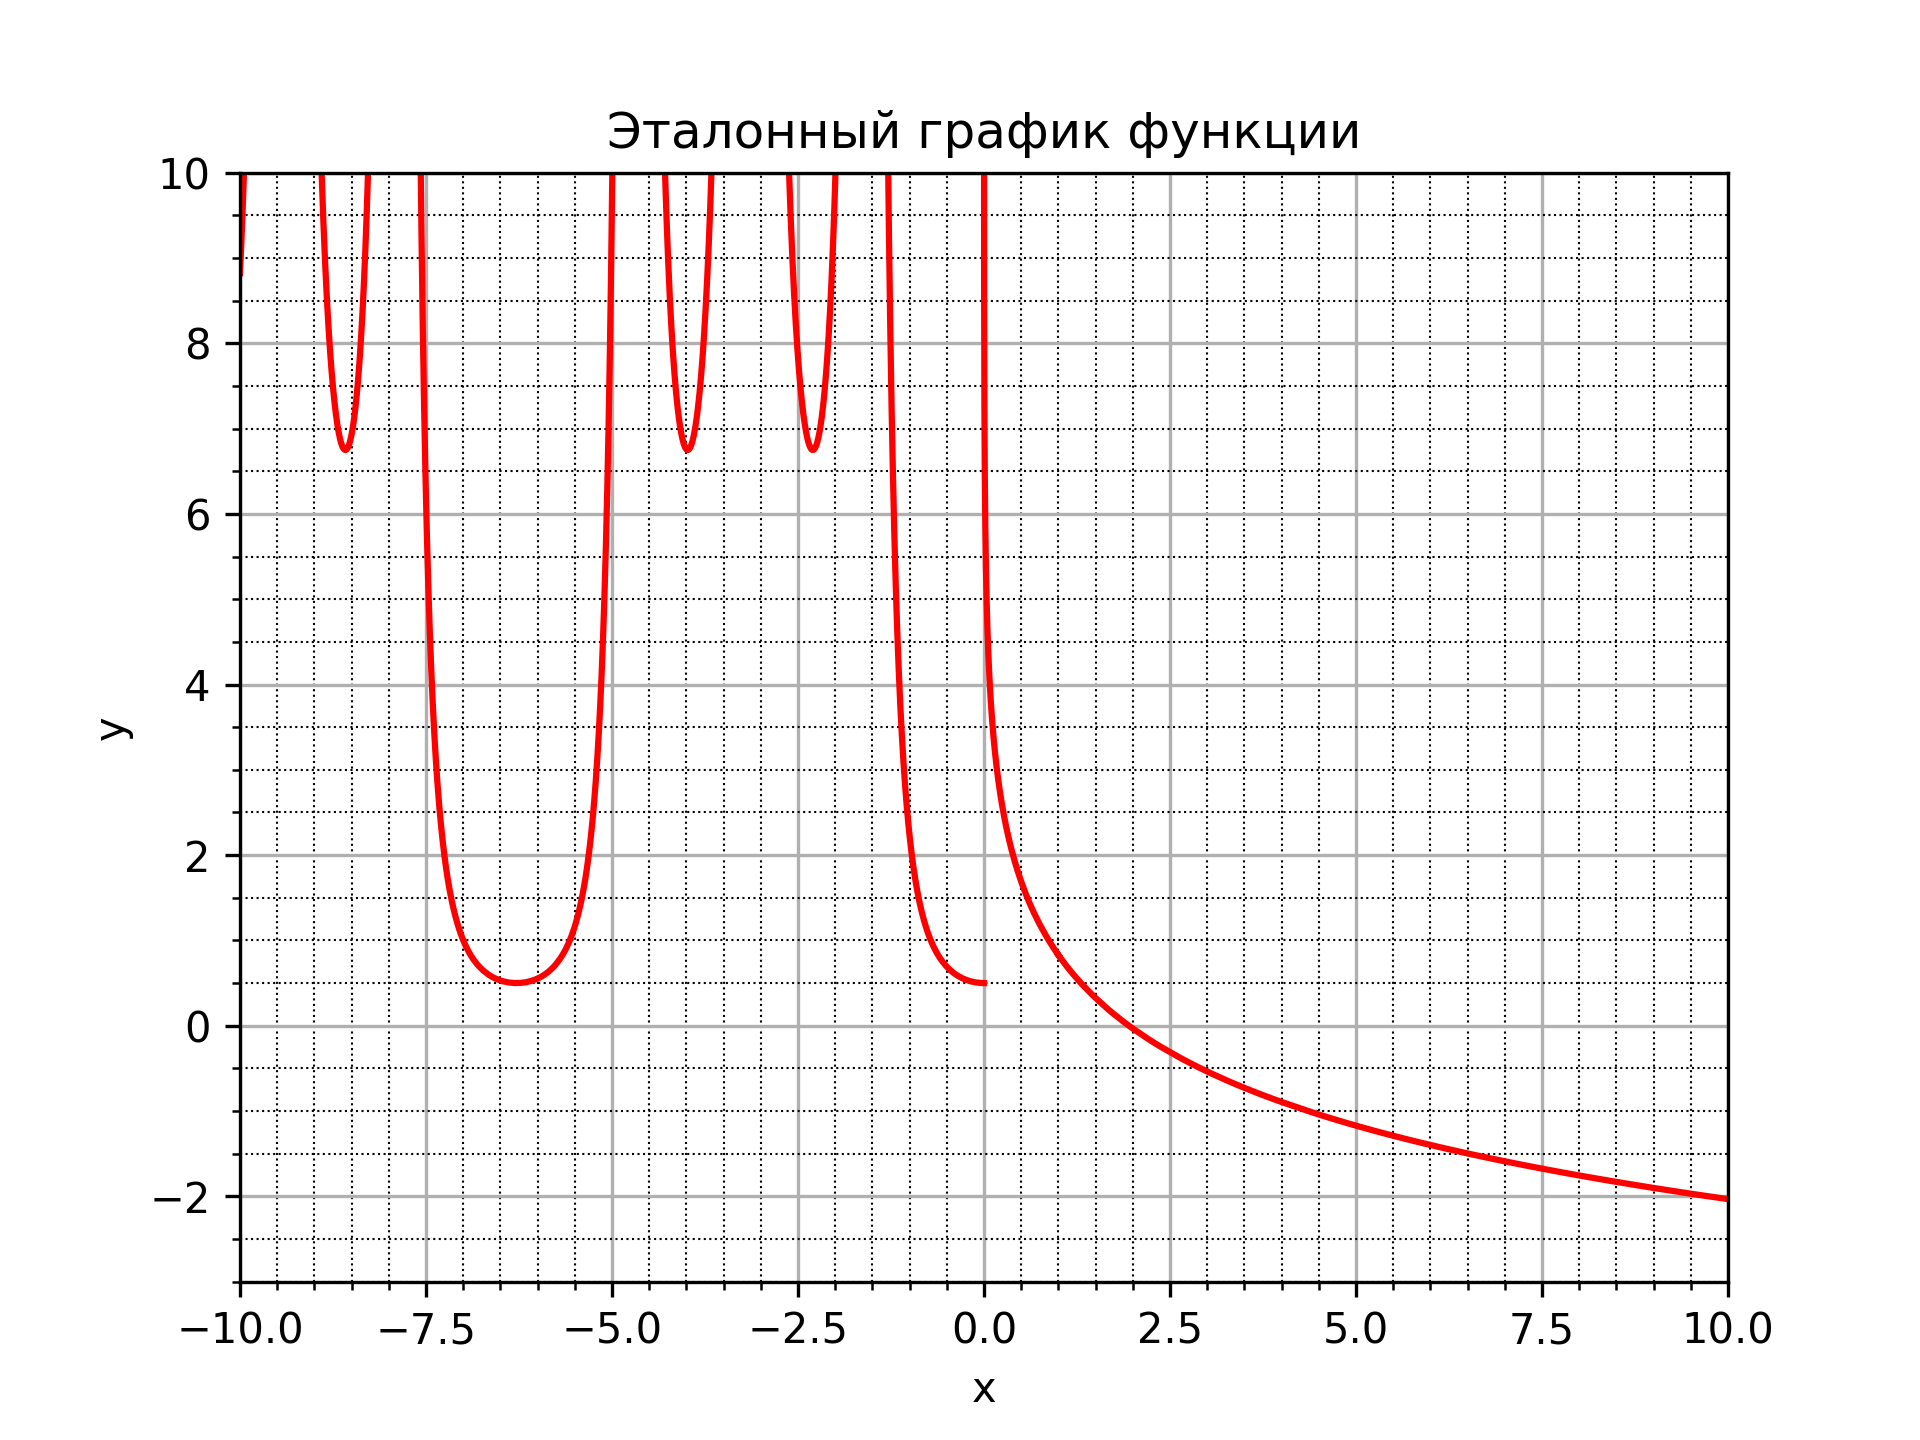
\includegraphics[width=\textwidth]{image/myFuncIdeal.png}
\end{figure}
Отличие только в количестве точек.

\subsubsection*{Графики других функций:}
\begin{figure}[H]
    \centering
    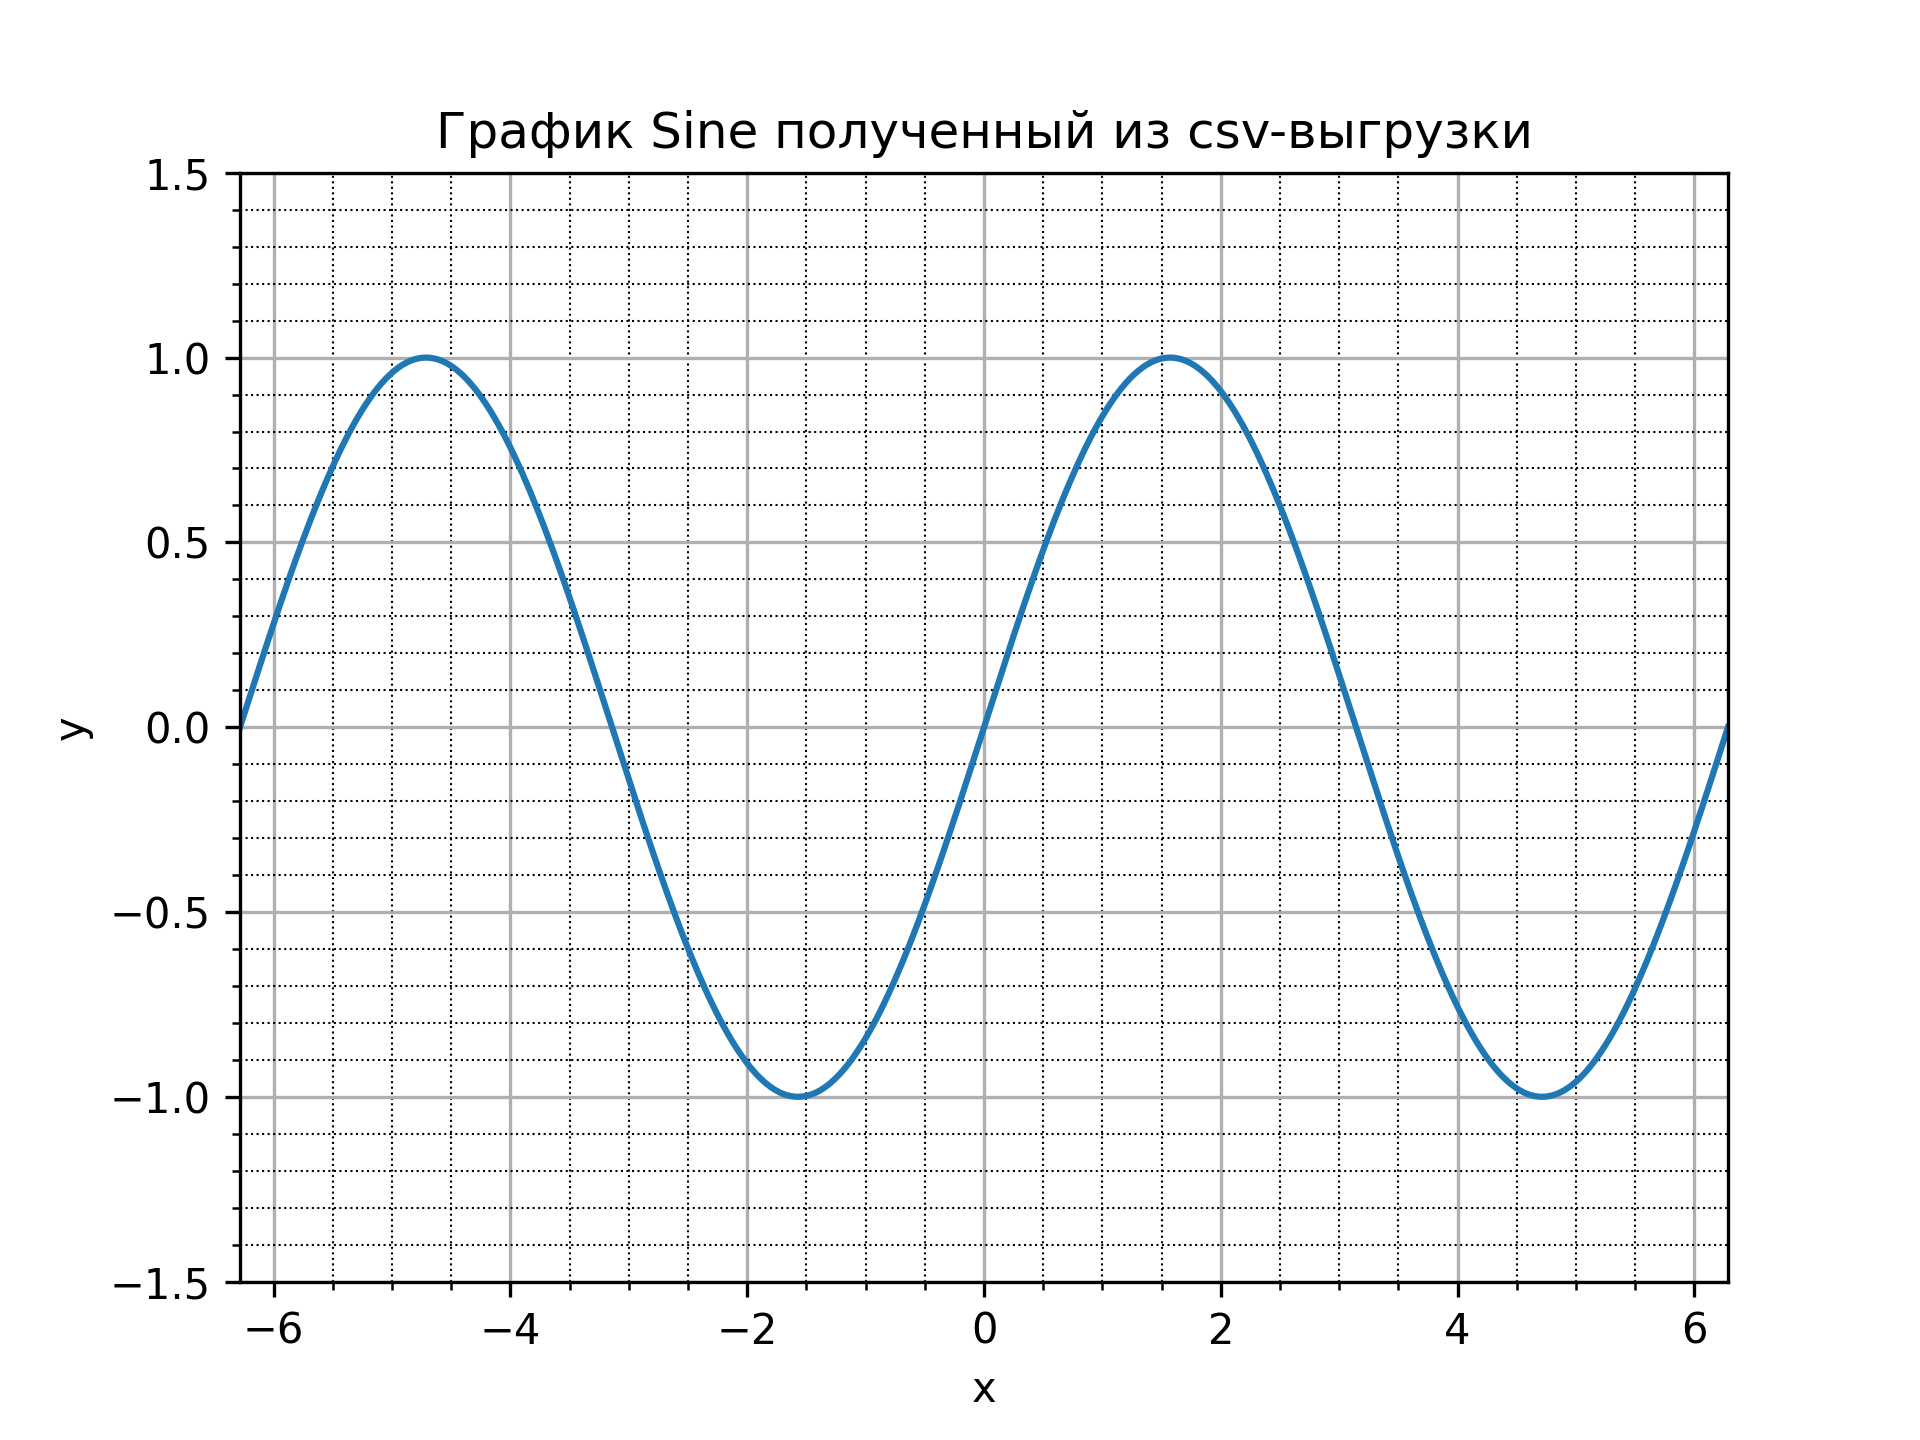
\includegraphics[width=\textwidth]{image/Sine.png}
\end{figure}
\begin{figure}[H]
    \centering
    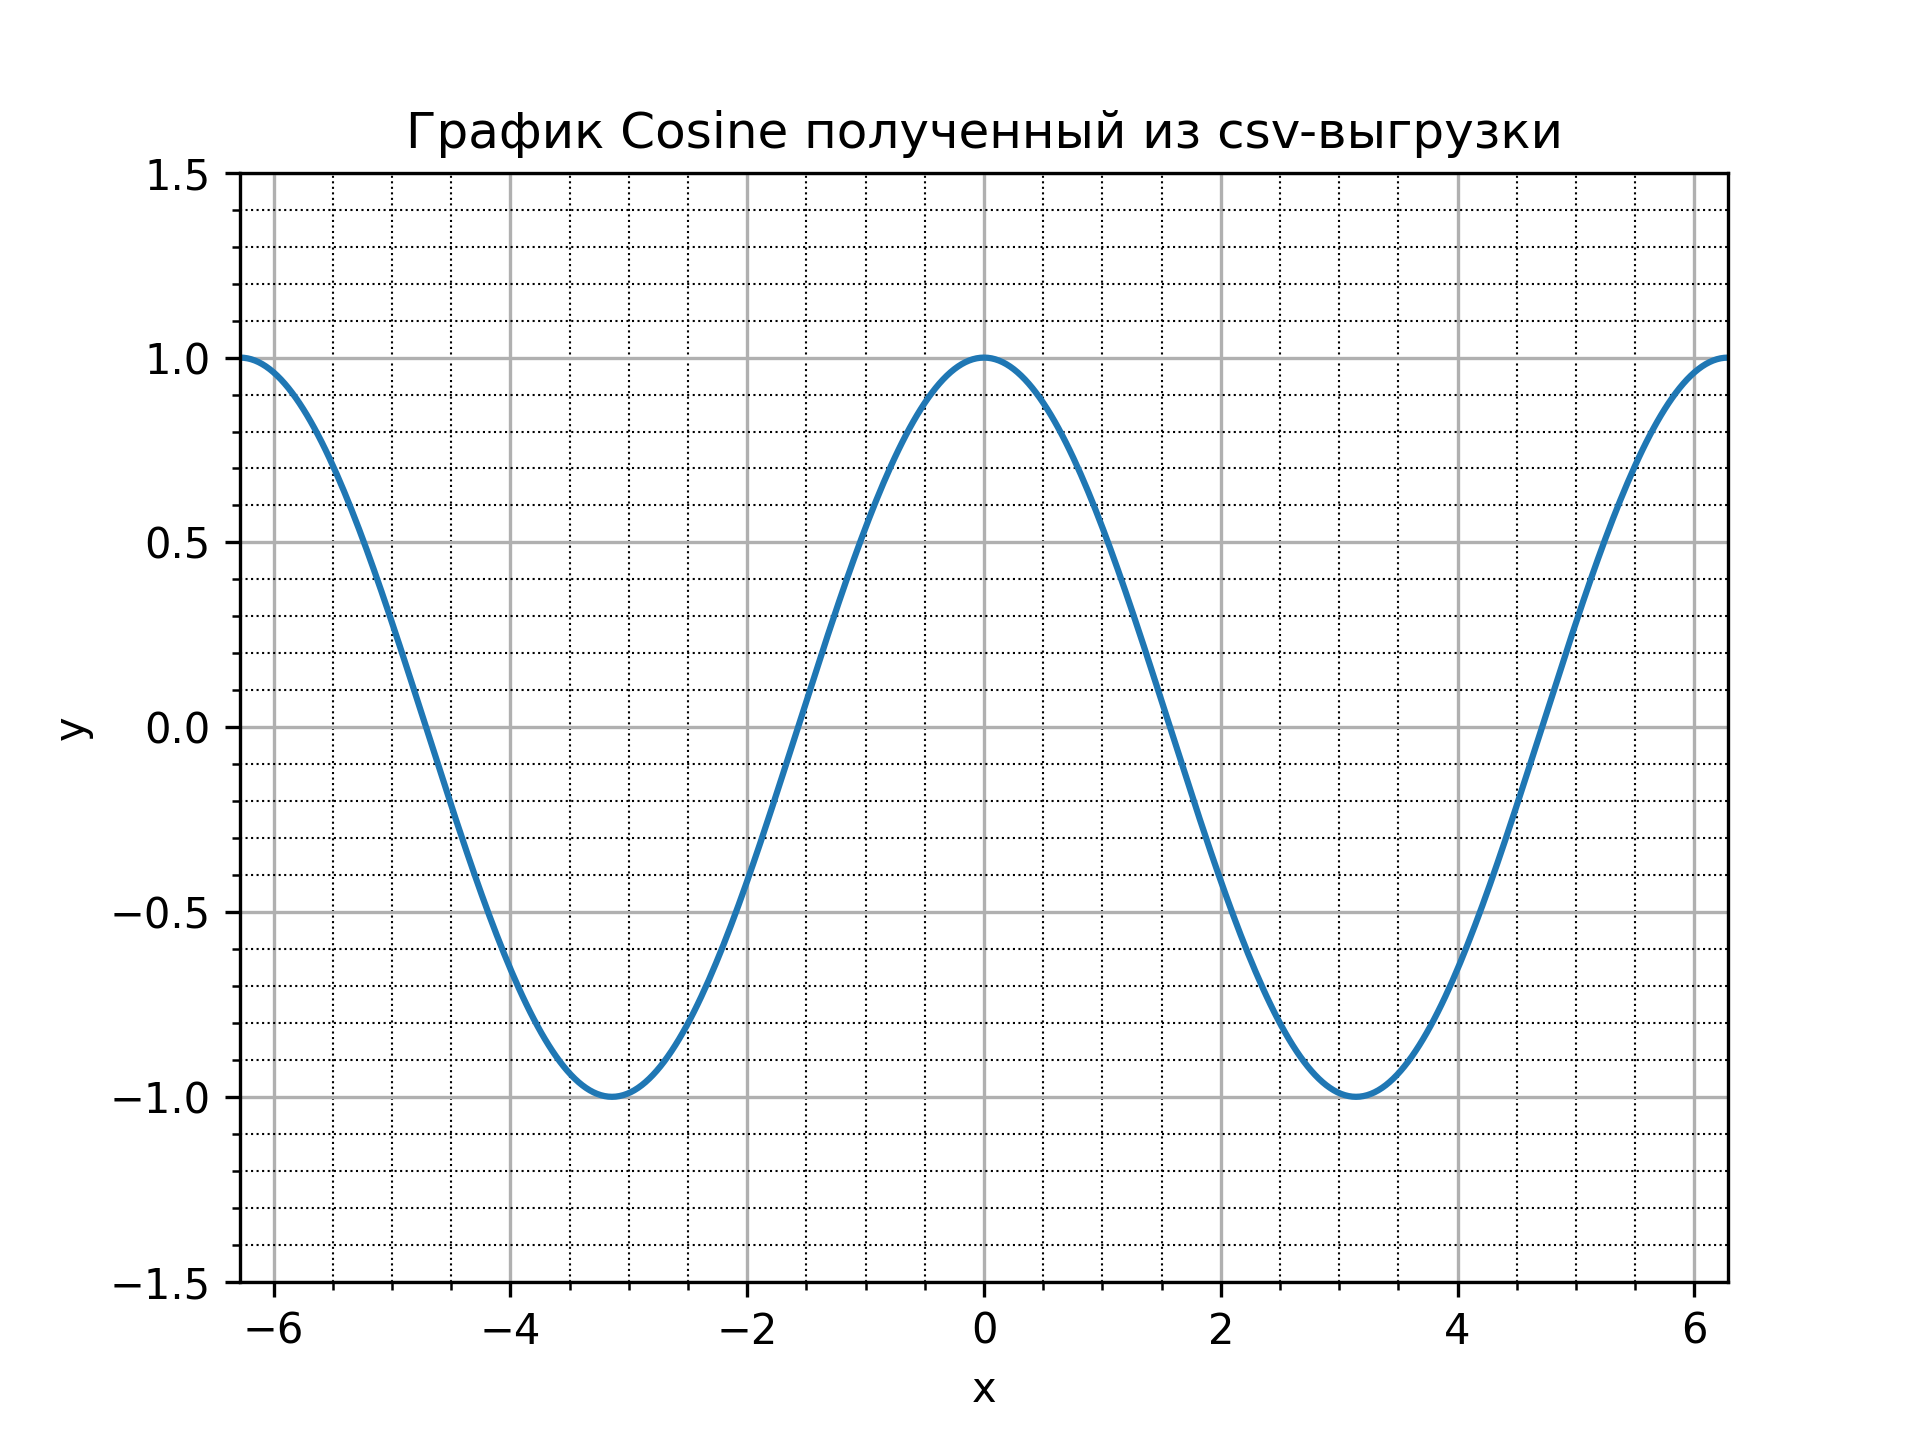
\includegraphics[width=\textwidth]{image/Cosine.png}
\end{figure}
\begin{figure}[H]
    \centering
    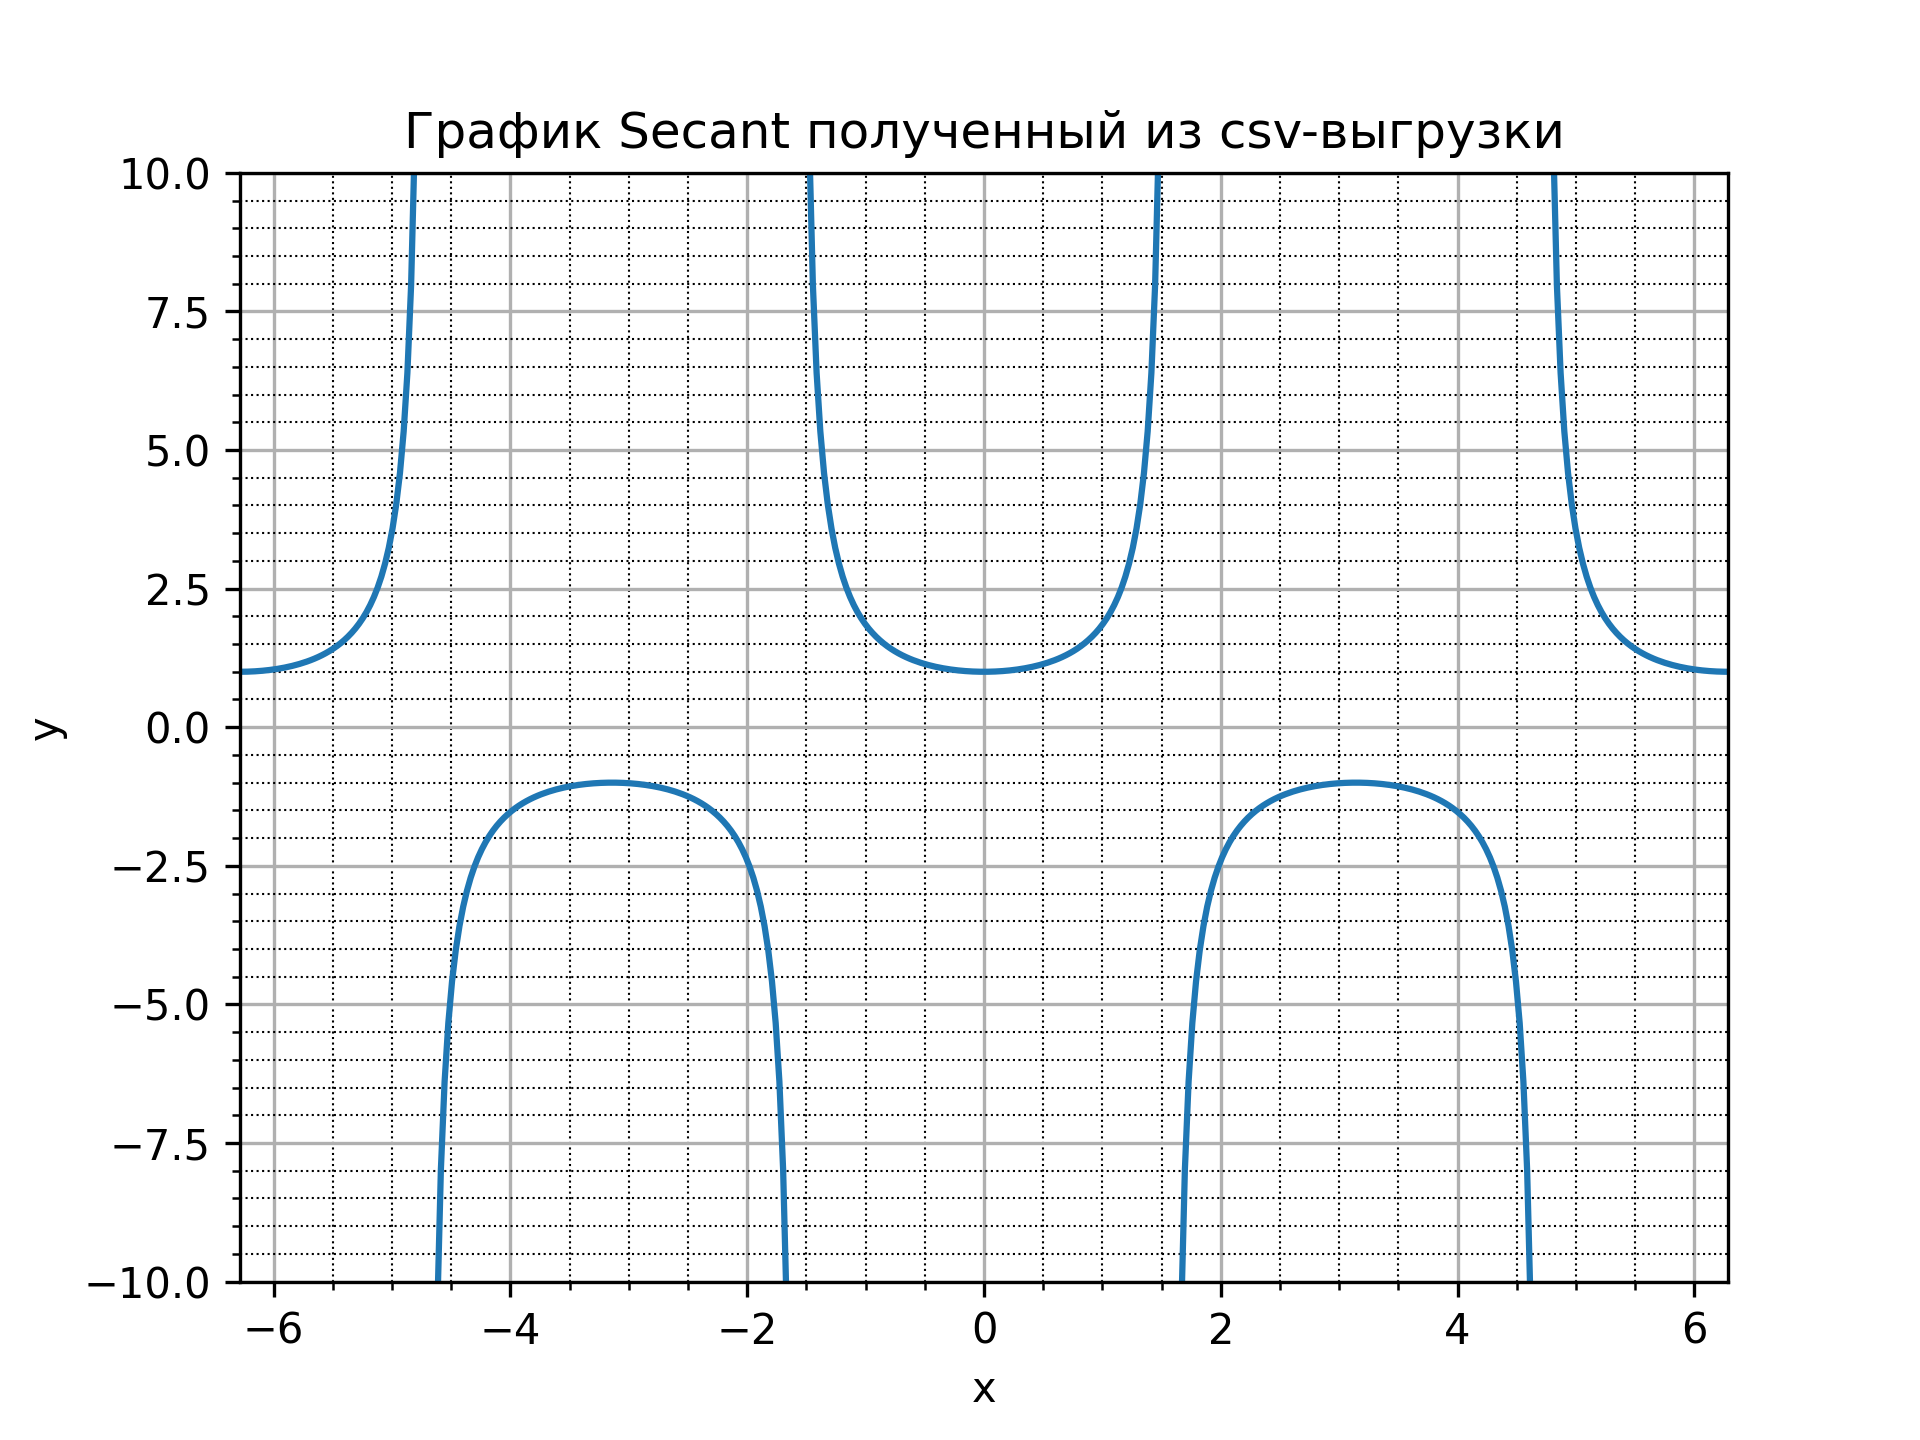
\includegraphics[width=\textwidth]{image/Secant.png}
\end{figure}
\begin{figure}[H]
    \centering
    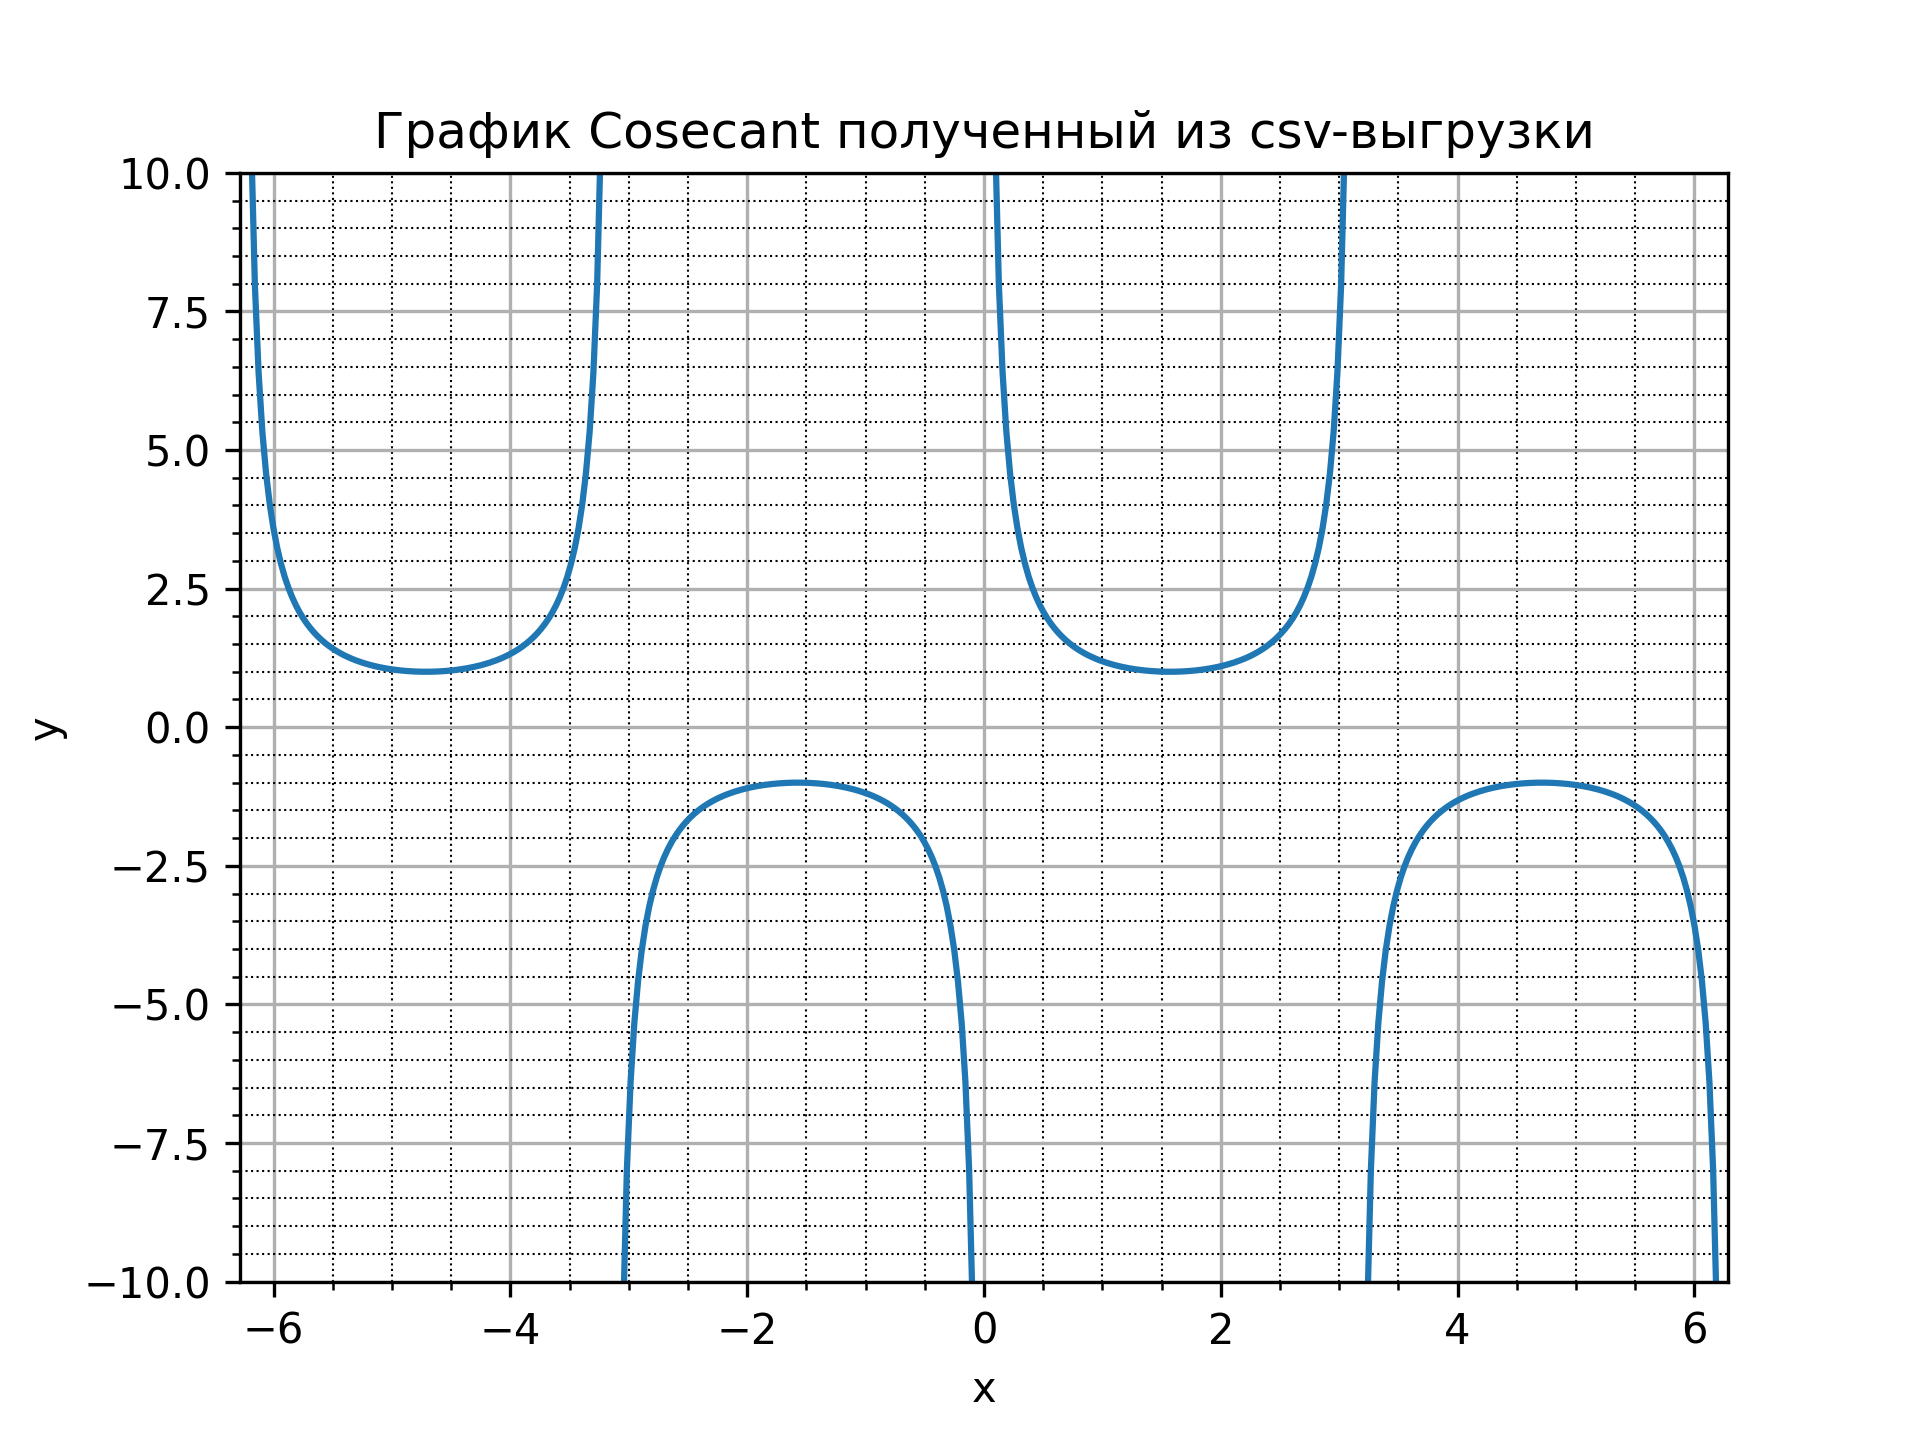
\includegraphics[width=\textwidth]{image/Cosecant.png}
\end{figure}
\begin{figure}[H]
    \centering
    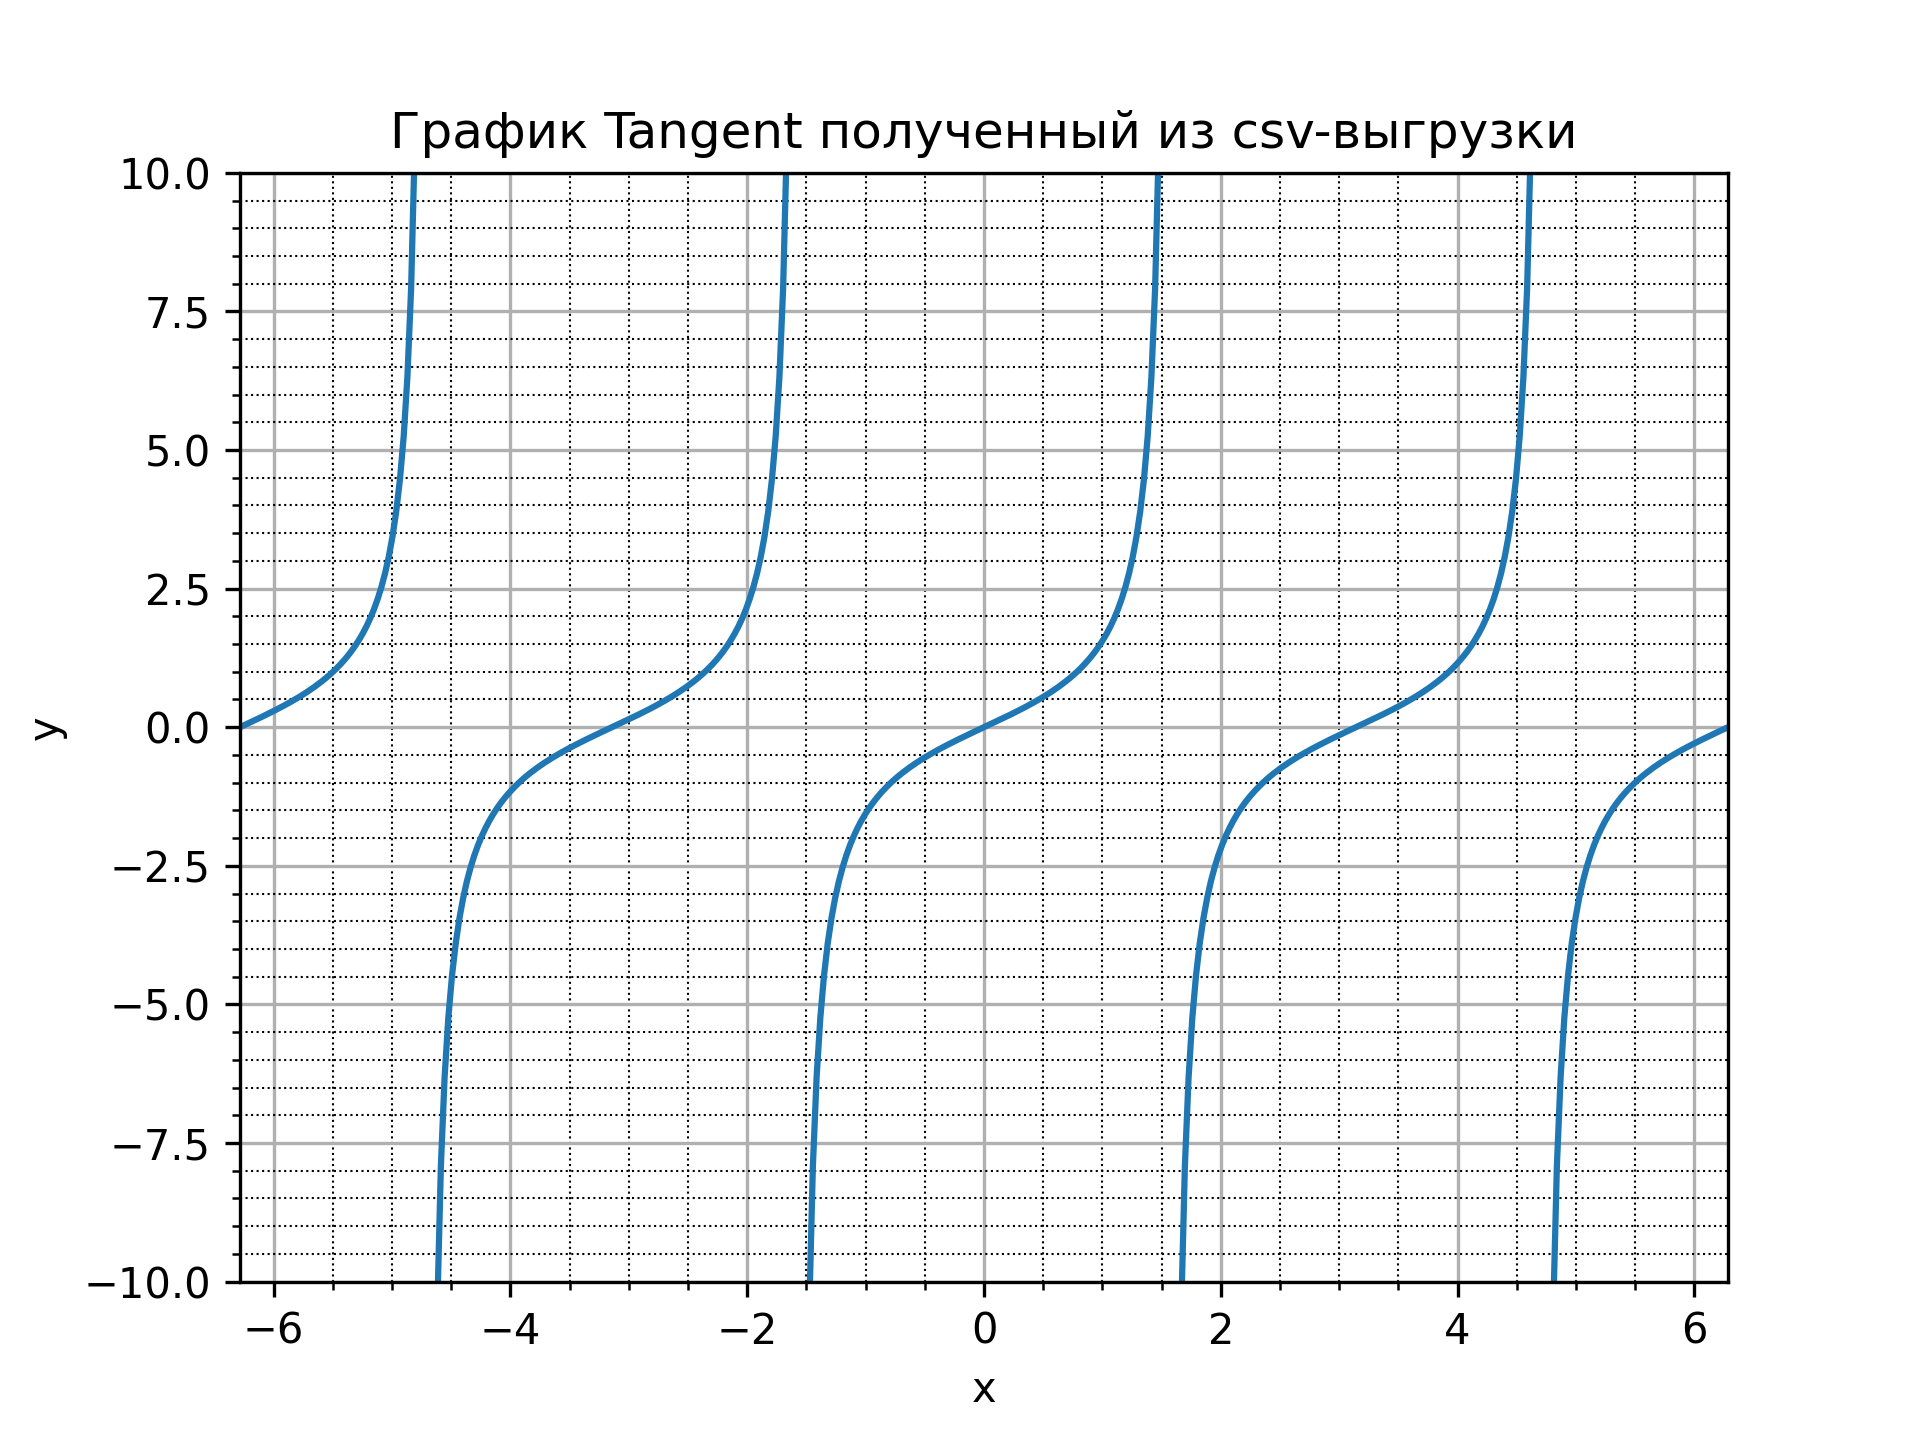
\includegraphics[width=\textwidth]{image/Tangent.png}
\end{figure}
\begin{figure}[H]
    \centering
    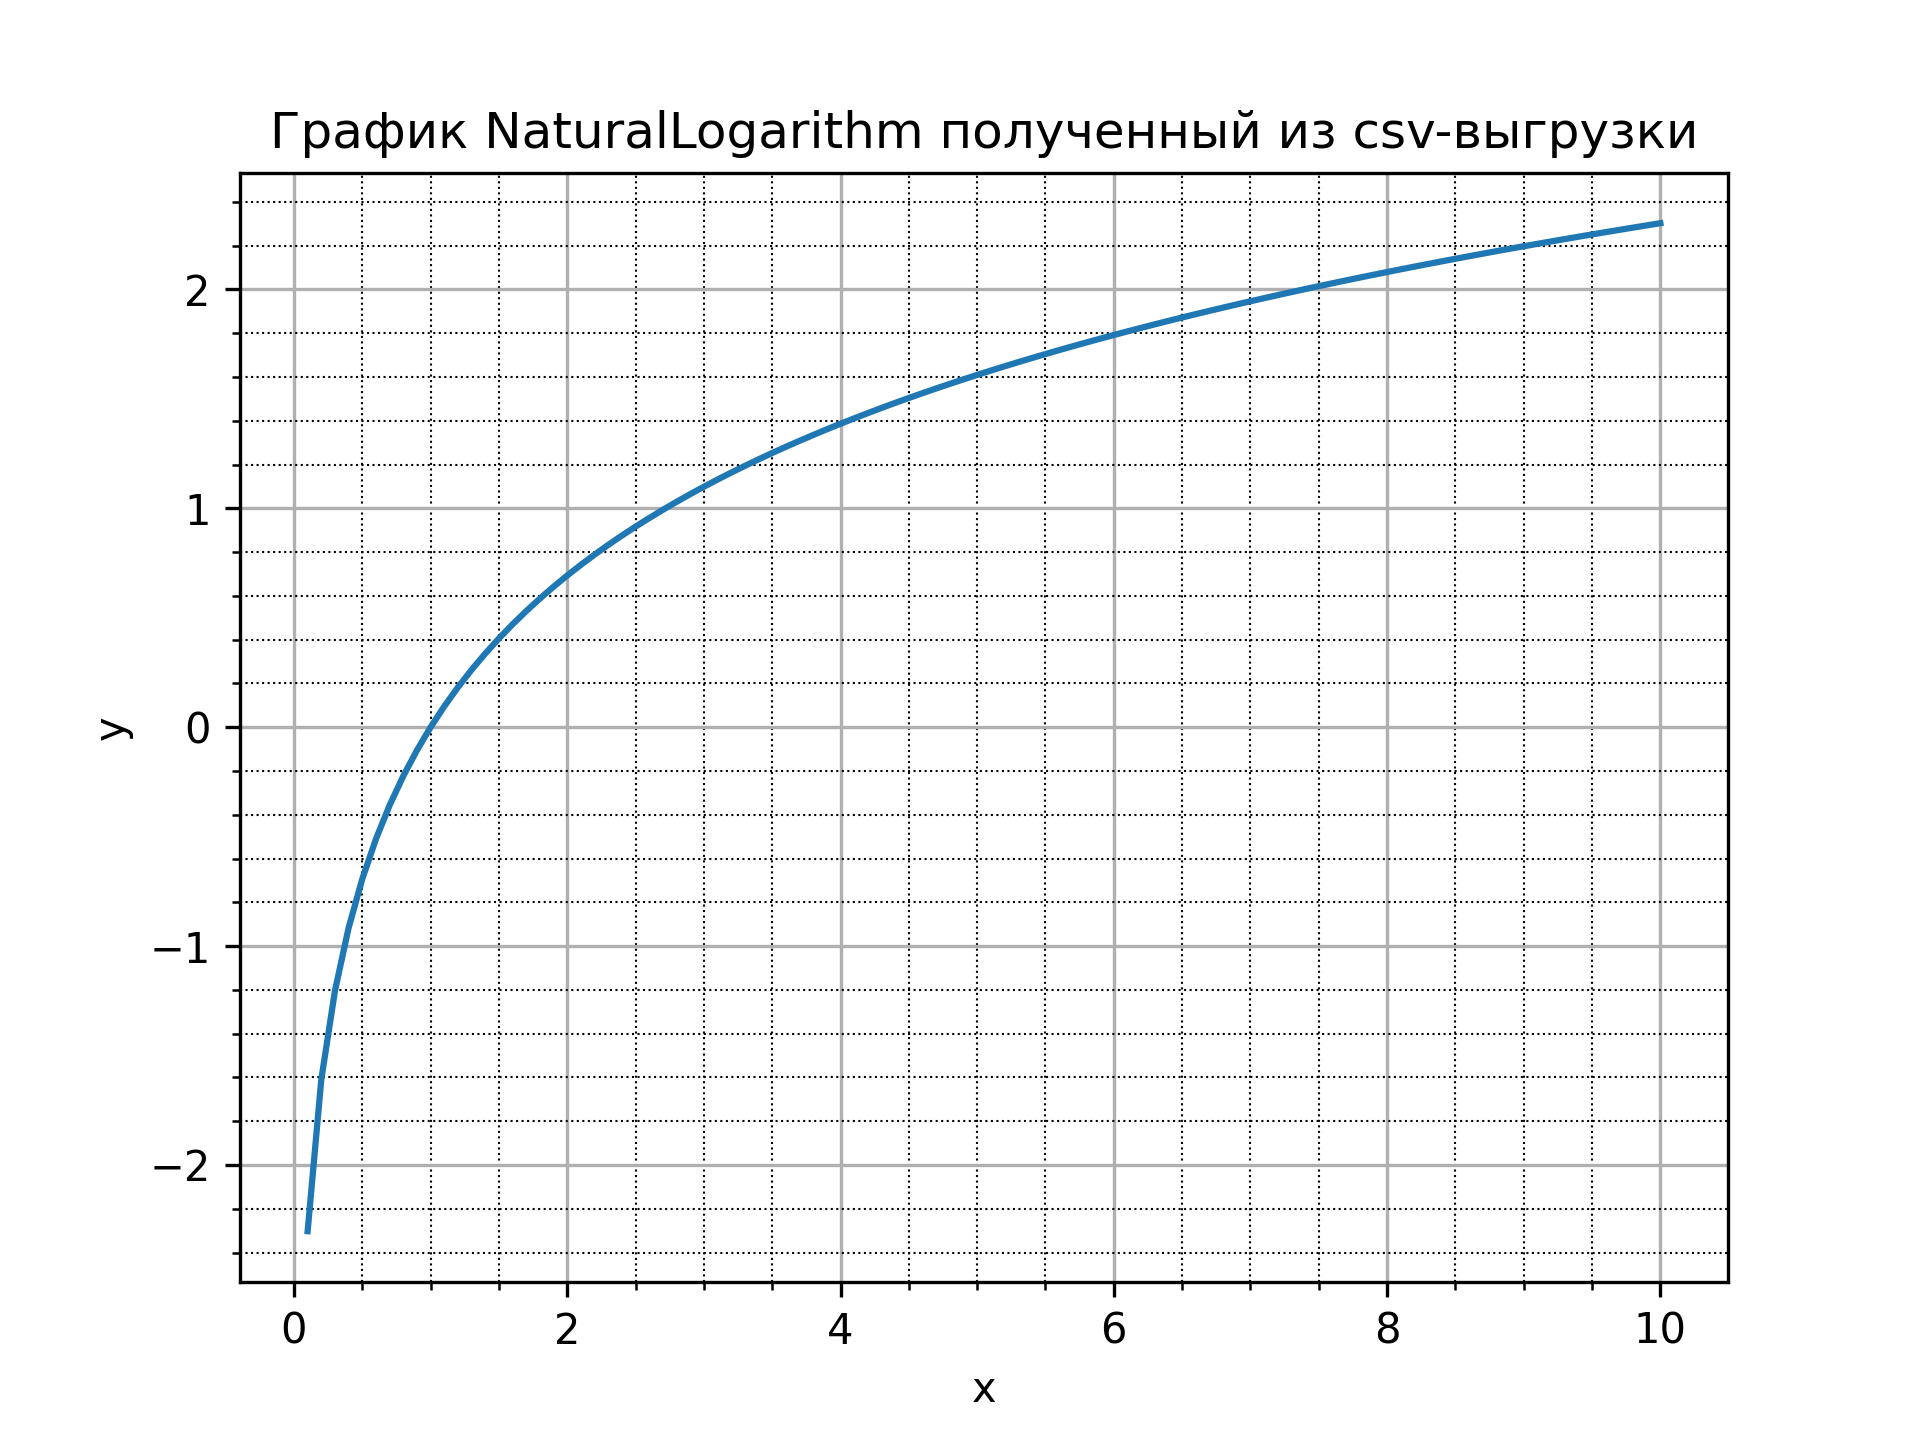
\includegraphics[width=\textwidth]{image/NaturalLogarithm.png}
\end{figure}
\begin{figure}[H]
    \centering
    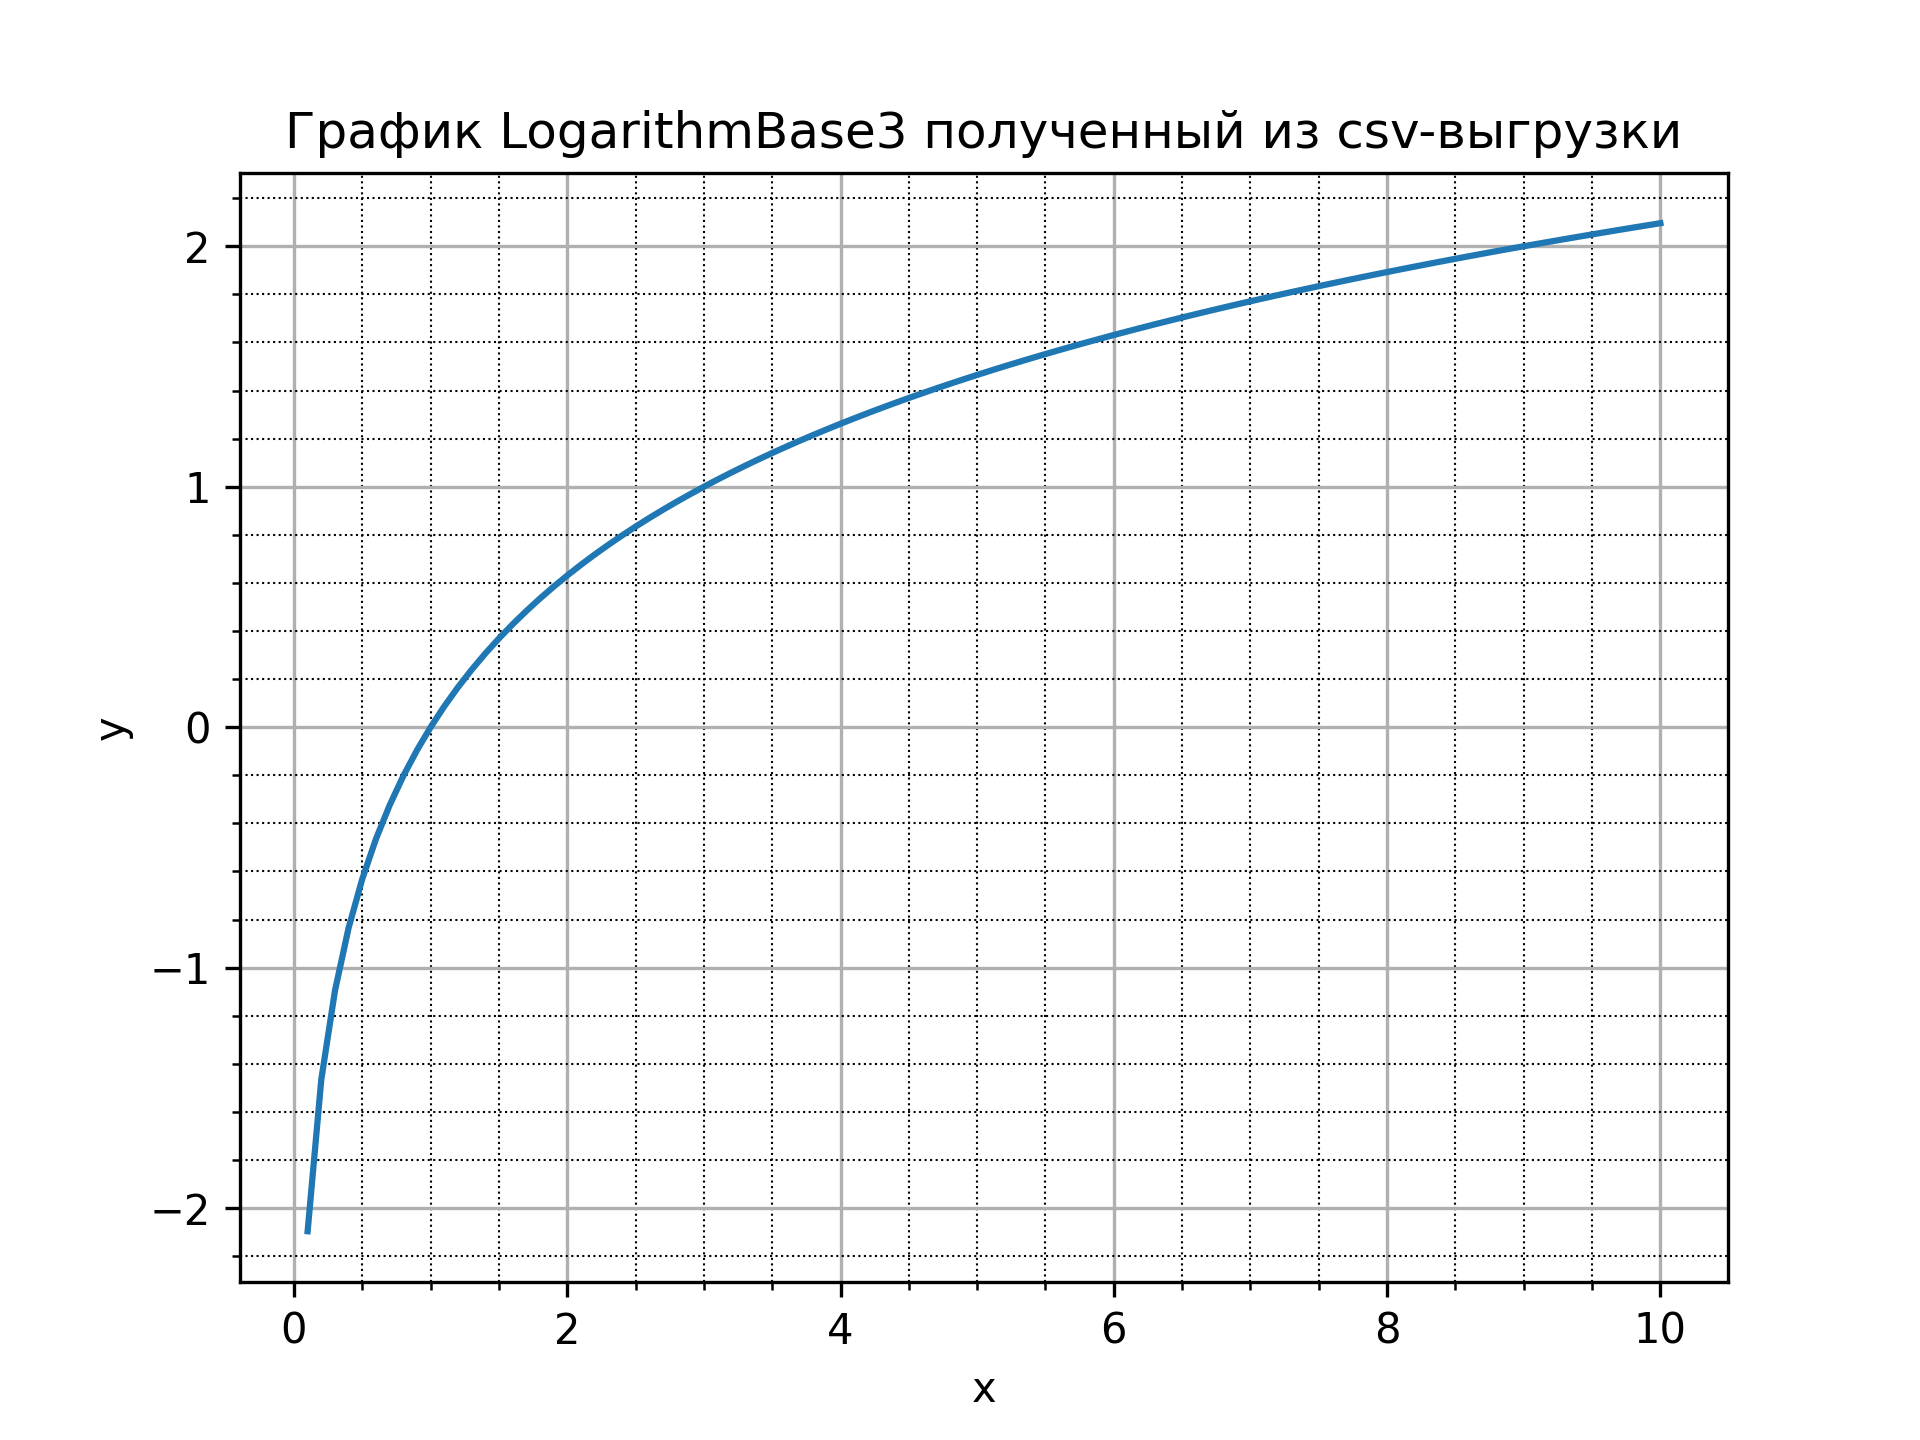
\includegraphics[width=\textwidth]{image/LogarithmBase3.png}
\end{figure}
\begin{figure}[H]
    \centering
    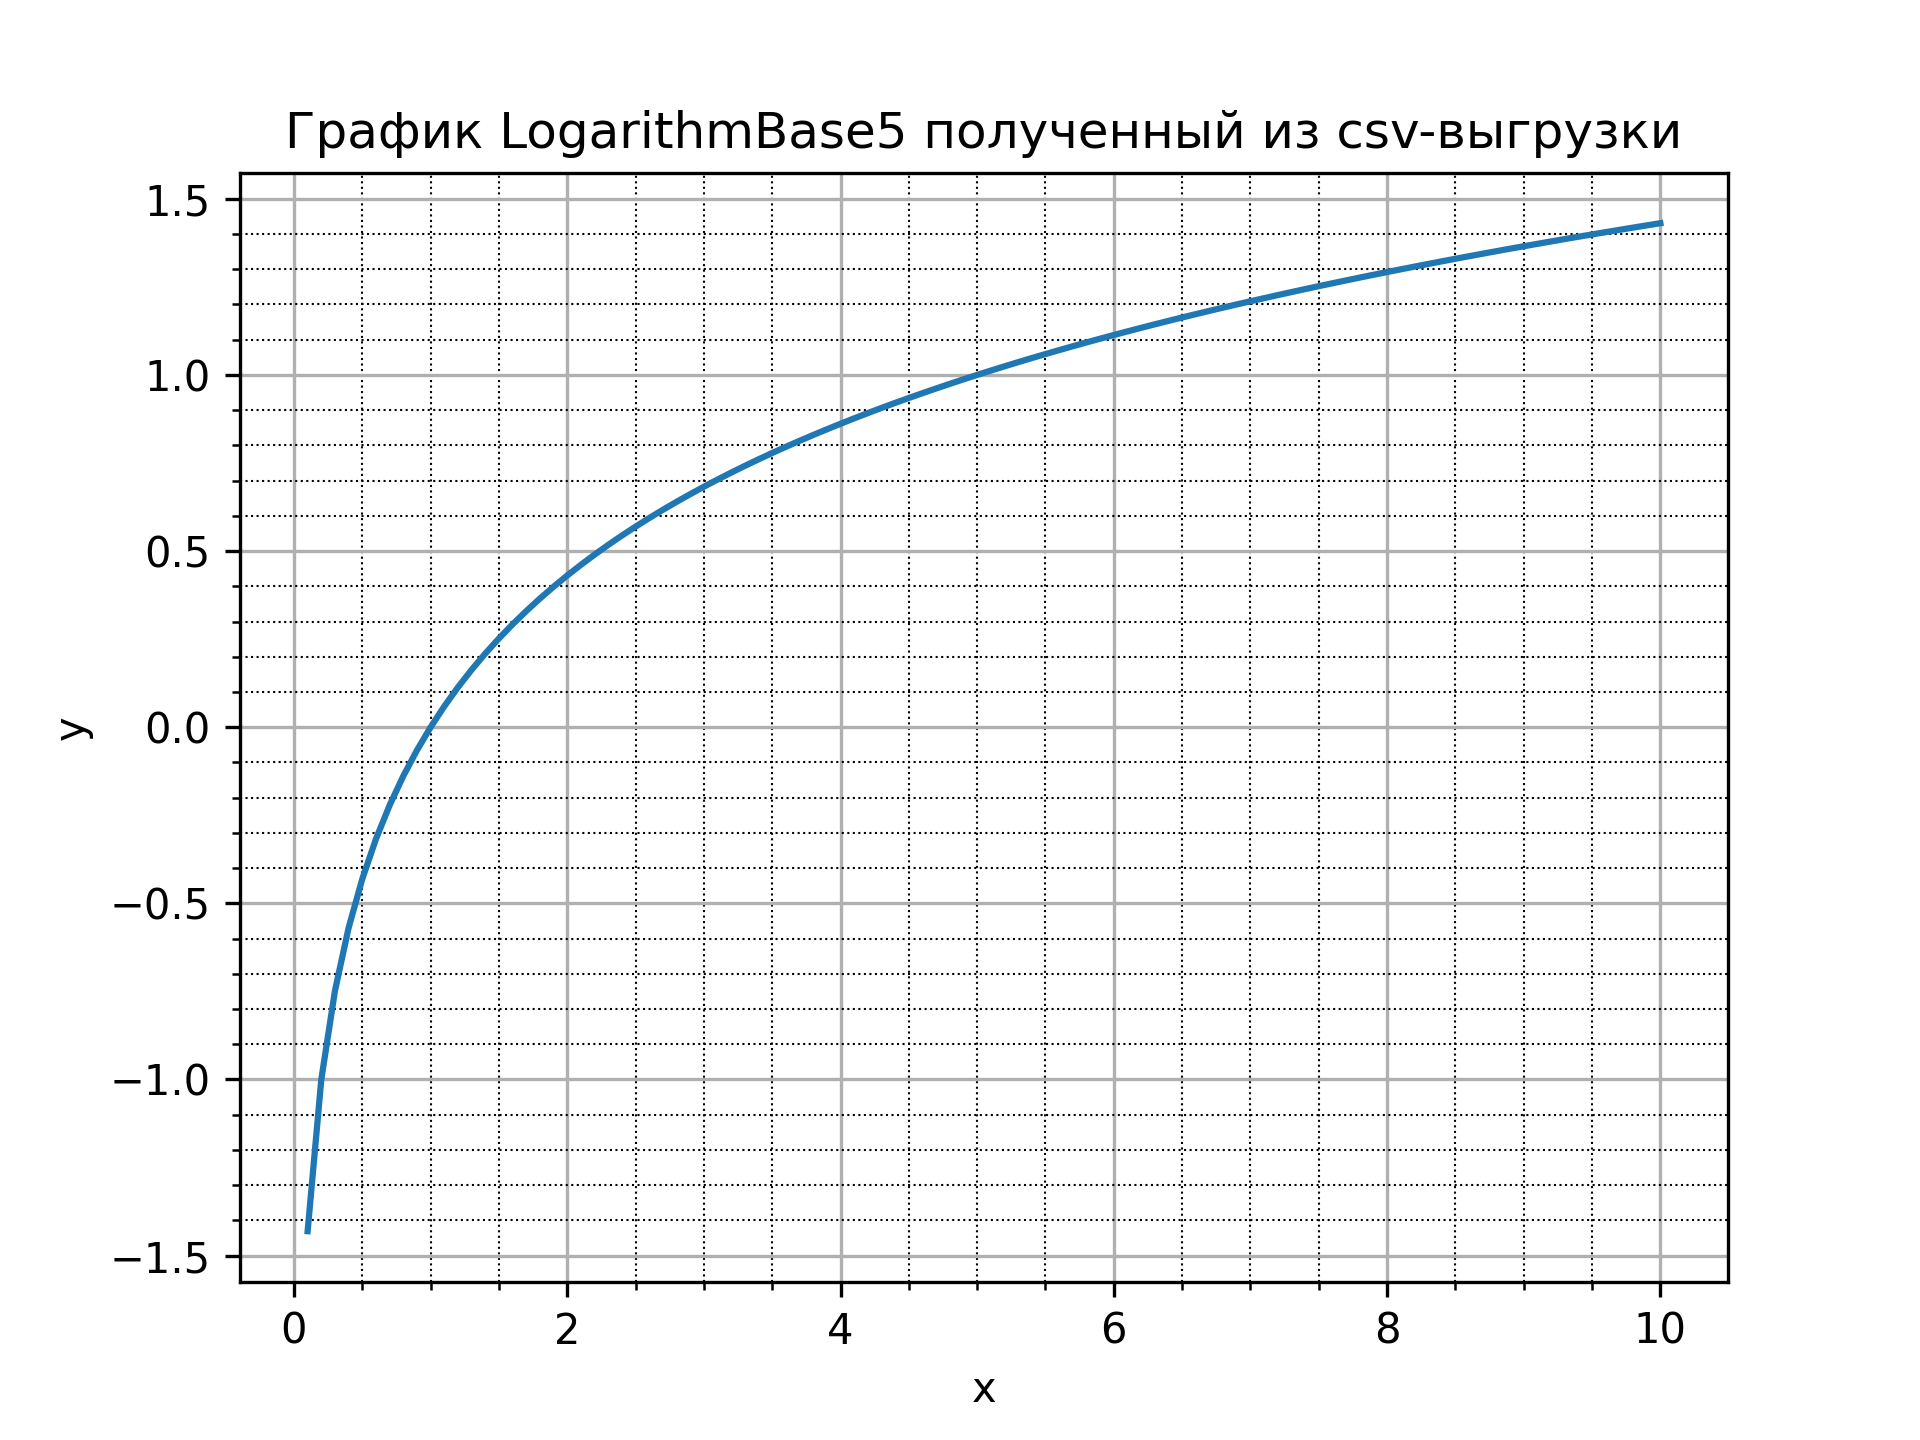
\includegraphics[width=\textwidth]{image/LogarithmBase5.png}
\end{figure}
\section*{Исходный код}
Можно просмотреть в моём GitHub: \href{https://github.com/AaLexUser/Software-testing}{https://github.com/AaLexUser/Software-testing}
\section*{Выводы по работе.}
В ходе выполнения данной лабораторной работы я провел интеграционное тестирование разработанной программы и изучил работу классов-заглушек на примере Mockito.
\end{document}